%File: anonymous-submission-latex-2026.tex
\documentclass[letterpaper]{article} % DO NOT CHANGE THIS
\usepackage[submission]{aaai2026}  % DO NOT CHANGE THIS
\usepackage{times}  % DO NOT CHANGE THIS
\usepackage{helvet}  % DO NOT CHANGE THIS
\usepackage{courier}  % DO NOT CHANGE THIS
\usepackage[hyphens]{url}  % DO NOT CHANGE THIS
\usepackage{graphicx} % DO NOT CHANGE THIS
\urlstyle{rm} % DO NOT CHANGE THIS
\def\UrlFont{\rm}  % DO NOT CHANGE THIS
\usepackage{natbib}  % DO NOT CHANGE THIS AND DO NOT ADD ANY OPTIONS TO IT
\usepackage{caption} % DO NOT CHANGE THIS AND DO NOT ADD ANY OPTIONS TO IT
\frenchspacing  % DO NOT CHANGE THIS
\setlength{\pdfpagewidth}{8.5in} % DO NOT CHANGE THIS
\setlength{\pdfpageheight}{11in} % DO NOT CHANGE THIS
%
\usepackage{algorithm}
\usepackage{algorithmic}

% These are are recommended to typeset listings but not required. See the subsubsection on listing. Remove this block if you don't have listings in your paper.
\usepackage{newfloat}
\usepackage{listings}
\DeclareCaptionStyle{ruled}{labelfont=normalfont,labelsep=colon,strut=off} % DO NOT CHANGE THIS
\lstset{%
	basicstyle={\footnotesize\ttfamily},% footnotesize acceptable for monospace
	numbers=left,numberstyle=\footnotesize,xleftmargin=2em,% show line numbers, remove this entire line if you don't want the numbers.
	aboveskip=0pt,belowskip=0pt,%
	showstringspaces=false,tabsize=2,breaklines=true}
\floatstyle{ruled}
\newfloat{listing}{tb}{lst}{}
\floatname{listing}{Listing}
%
% Keep the \pdfinfo as shown here. There's no need
% for you to add the /Title and /Author tags.
\pdfinfo{
/TemplateVersion (2026.1)
}



\usepackage{subcaption}
\usepackage{paralist}
\usepackage{bm}
\usepackage{mathtools}
\usepackage{amsmath}
\usepackage{amssymb}
\usepackage{multirow}
\usepackage{booktabs}
\usepackage{xcolor}
\usepackage{makecell}


% DISALLOWED PACKAGES
% \usepackage{authblk} -- This package is specifically forbidden
% \usepackage{balance} -- This package is specifically forbidden
% \usepackage{color (if used in text)
% \usepackage{CJK} -- This package is specifically forbidden
% \usepackage{float} -- This package is specifically forbidden
% \usepackage{flushend} -- This package is specifically forbidden
% \usepackage{fontenc} -- This package is specifically forbidden
% \usepackage{fullpage} -- This package is specifically forbidden
% \usepackage{geometry} -- This package is specifically forbidden
% \usepackage{grffile} -- This package is specifically forbidden
% \usepackage{hyperref} -- This package is specifically forbidden
% \usepackage{navigator} -- This package is specifically forbidden
% (or any other package that embeds links such as navigator or hyperref)
% \indentfirst} -- This package is specifically forbidden
% \layout} -- This package is specifically forbidden
% \multicol} -- This package is specifically forbidden
% \nameref} -- This package is specifically forbidden
% \usepackage{savetrees} -- This package is specifically forbidden
% \usepackage{setspace} -- This package is specifically forbidden
% \usepackage{stfloats} -- This package is specifically forbidden
% \usepackage{tabu} -- This package is specifically forbidden
% \usepackage{titlesec} -- This package is specifically forbidden
% \usepackage{tocbibind} -- This package is specifically forbidden
% \usepackage{ulem} -- This package is specifically forbidden
% \usepackage{wrapfig} -- This package is specifically forbidden
% DISALLOWED COMMANDS
% \nocopyright -- Your paper will not be published if you use this command
% \addtolength -- This command may not be used
% \balance -- This command may not be used
% \baselinestretch -- Your paper will not be published if you use this command
% \clearpage -- No page breaks of any kind may be used for the final version of your paper
% \columnsep -- This command may not be used
% \newpage -- No page breaks of any kind may be used for the final version of your paper
% \pagebreak -- No page breaks of any kind may be used for the final version of your paperr
% \pagestyle -- This command may not be used
% \tiny -- This is not an acceptable font size.
% \vspace{- -- No negative value may be used in proximity of a caption, figure, table, section, subsection, subsubsection, or reference
% \vskip{- -- No negative value may be used to alter spacing above or below a caption, figure, table, section, subsection, subsubsection, or reference

\setcounter{secnumdepth}{2} %May be changed to 1 or 2 if section numbers are desired.

% The file aaai2026.sty is the style file for AAAI Press
% proceedings, working notes, and technical reports.
%

% Title

% Your title must be in mixed case, not sentence case.
% That means all verbs (including short verbs like be, is, using,and go),
% nouns, adverbs, adjectives should be capitalized, including both words in hyphenated terms, while
% articles, conjunctions, and prepositions are lower case unless they
% directly follow a colon or long dash
\title{Improving Human-Robot Teamwork in Urban Search and Rescue Through Knowledge Graph-Based Episodic Memory Learning}
\author{
    %Authors
    % All authors must be in the same font size and format.
    Written by AAAI Press Staff\textsuperscript{\rm 1}\thanks{With help from the AAAI Publications Committee.}\\
    AAAI Style Contributions by Pater Patel Schneider,
    Sunil Issar,\\
    J. Scott Penberthy,
    George Ferguson,
    Hans Guesgen,
    Francisco Cruz\equalcontrib,
    Marc Pujol-Gonzalez\equalcontrib
}
\affiliations{
    %Afiliations
    \textsuperscript{\rm 1}Association for the Advancement of Artificial Intelligence\\
    % If you have multiple authors and multiple affiliations
    % use superscripts in text and roman font to identify them.
    % For example,

    % Sunil Issar\textsuperscript{\rm 2},
    % J. Scott Penberthy\textsuperscript{\rm 3},
    % George Ferguson\textsuperscript{\rm 4},
    % Hans Guesgen\textsuperscript{\rm 5}
    % Note that the comma should be placed after the superscript

    1101 Pennsylvania Ave, NW Suite 300\\
    Washington, DC 20004 USA\\
    % email address must be in roman text type, not monospace or sans serif
    proceedings-questions@aaai.org
%
% See more examples next
}

%Example, Single Author, ->> remove \iffalse,\fi and place them surrounding AAAI title to use it
\iffalse
\title{My Publication Title --- Single Author}
\author {
    Author Name
}
\affiliations{
    Affiliation\\
    Affiliation Line 2\\
    name@example.com
}
\fi

\iffalse
%Example, Multiple Authors, ->> remove \iffalse,\fi and place them surrounding AAAI title to use it
\title{My Publication Title --- Multiple Authors}
\author {
    % Authors
    First Author Name\textsuperscript{\rm 1},
    Second Author Name\textsuperscript{\rm 2},
    Third Author Name\textsuperscript{\rm 1}
}
\affiliations {
    % Affiliations
    \textsuperscript{\rm 1}Affiliation 1\\
    \textsuperscript{\rm 2}Affiliation 2\\
    firstAuthor@affiliation1.com, secondAuthor@affilation2.com, thirdAuthor@affiliation1.com
}
\fi


% REMOVE THIS: bibentry
% This is only needed to show inline citations in the guidelines document. You should not need it and can safely delete it.
\usepackage{bibentry}
% END REMOVE bibentry

\begin{document}

\maketitle

\begin{abstract}
Effective human–robot teamwork demands that robots adapt on the fly to volatile, co‑evolving human behavior. In MATRX USAR simulations, performance rises when humans label and share collaboration patterns (CPs) with the robot via chat. This study aims to advance human-robot collaboration by developing an episodic long-term memory that integrates and maintains these patterns in a dedicated ontology-based Knowledge Graph (KG). We apply graph representation self-supervised learning to cluster these memories, identifying the most representative and effective experiences. Unlike previous approaches where robots start with an empty memory state, we initialize the robot’s memory with these insights, enabling it to retain knowledge. On 160 trials, seeding the robot with a single, automatically chosen CP lifts rescue success from 25.7\% to 41.3\% and cuts average task time by 283s.
\end{abstract}

% Uncomment the following to link to your code, datasets, an extended version or similar.
% You must keep this block between (not within) the abstract and the main body of the paper.
% \begin{links}
%     \link{Code}{https://aaai.org/example/code}
%     \link{Datasets}{https://aaai.org/example/datasets}
%     \link{Extended version}{https://aaai.org/example/extended-version}
% \end{links}

\section{Introduction}
\label{sec:introduction}


\begin{figure}[tb]
\centering
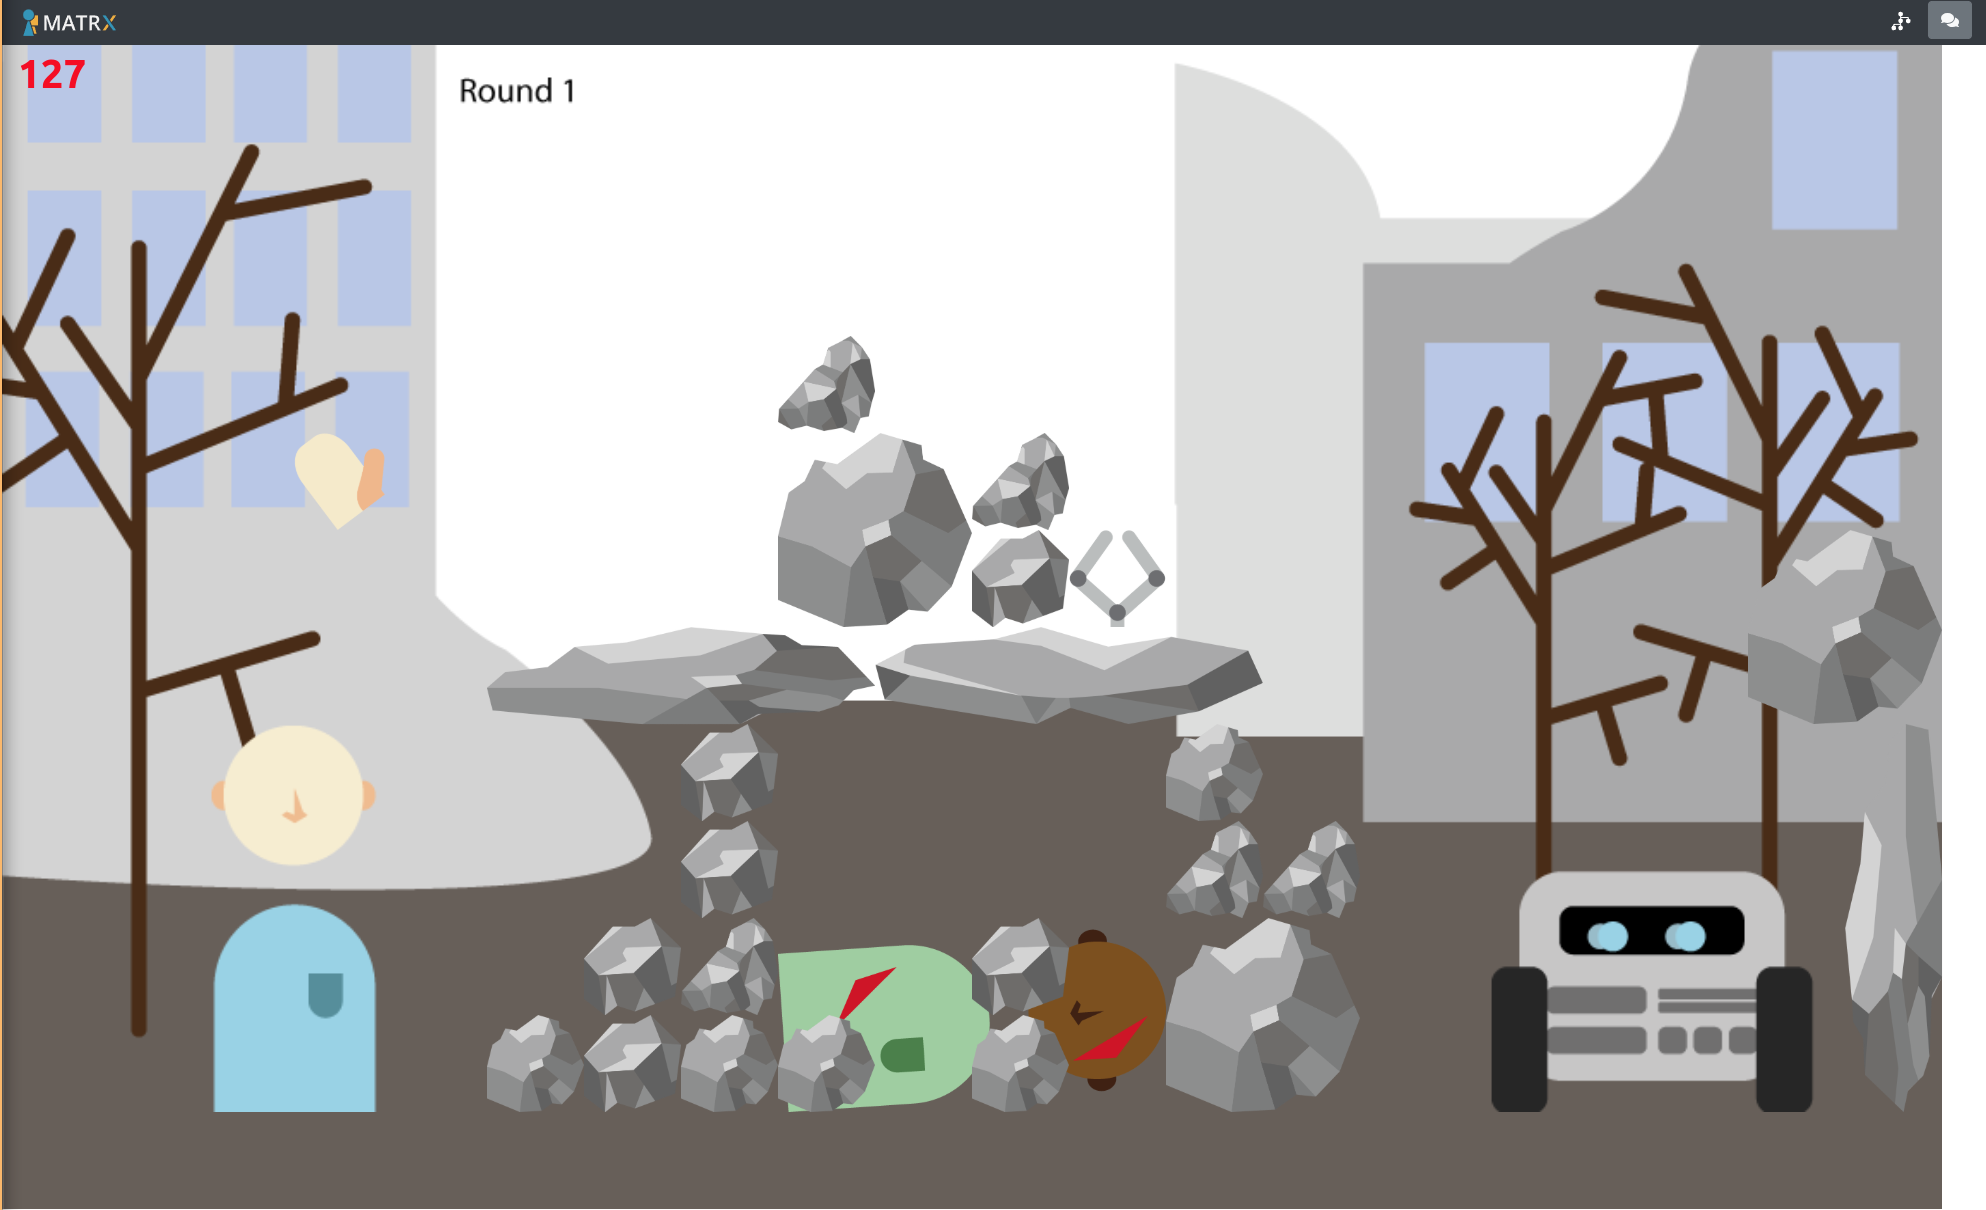
\includegraphics[width=\columnwidth]{figures/usar.png}
\caption{A screenshot of the MATRX USAR simulation. The human user is shown on the left, while the robot is on the right. In the upper right corner, users can click icons to define a collaboration pattern (CP) or open the chat interface.}
\label{fig:usar-main}
\end{figure}


\begin{figure}[tb]
\centering

\begin{subfigure}[b]{\columnwidth}
    \centering
    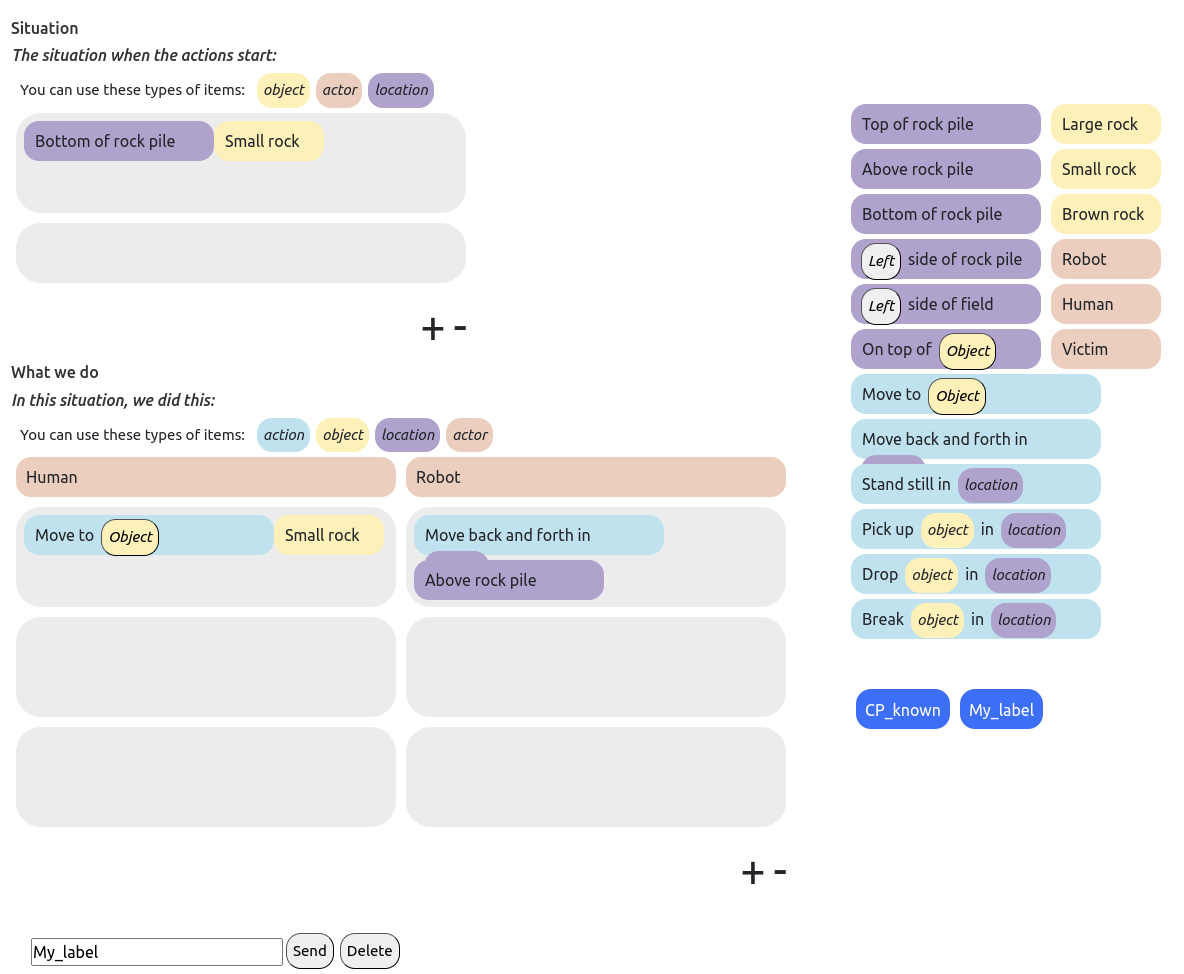
\includegraphics[width=\columnwidth]{figures/usar-cp.png}
    \caption{Users can drag and drop boxes (representing objects, actors, and locations) to document the emergent CPs they observe with the robot.}
    \label{fig:usar-cp}
\end{subfigure}

\vspace{1em}

\begin{subfigure}[b]{\columnwidth}
    % We manually create two columns within this subfigure:
    \begin{minipage}[b]{0.49\columnwidth}
        \centering
        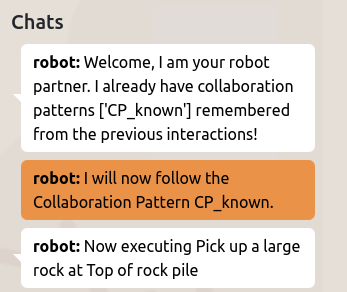
\includegraphics[width=\linewidth]{figures/usar-chat.png}
        % You can place a label here if needed, but typically
        % you'll label the entire subfigure (b) rather than just the image.
    \end{minipage}
    \hfill
    \begin{minipage}[b]{0.49\columnwidth}
        \small
        This chat interface enables the robot to communicate updates
        and inform human users about ongoing events.
    \end{minipage}

    \caption{The chat interface.}
    \label{fig:usar-chat}
\end{subfigure}

\caption{User interaction features in the MATRX USAR environment.
(a) The CP interface. (b) The chat interface.}
\label{fig:usar-interaction}
\end{figure}



Industrial robots usually work in static settings with little human contact~\cite{IFR2023}, but labour shortages and hazardous tasks are driving a shift toward teammate‑style autonomy~\cite{MarketsandMarkets2024}. For example, in disaster response, assistive robots are being developed to assist rescue teams by navigating debris, locating survivors, and delivering supplies in hazardous environments~\cite{Moosavi2024}.

Despite their potential, assistive robots face significant challenges in adapting to human partners. Unlike traditional robots operating in controlled environments, assistive robots must interpret human intentions, adjust to dynamic situations, and learn from past interactions. Human behavior is dynamic and variable, requiring assistive robots to process ambiguous cues, coordinate effectively, and refine their decision-making over time. These complexities make real-time adaptation difficult, highlighting the need for learning mechanisms that enable assistive robots to build and utilize memory from prior experiences.

One approach to studying human-robot collaboration is the MATRX Urban Search and Rescue (USAR) environment~\cite{matrx_2023,vanZoelen2021}, a virtual simulation where a collaborative robot and a human work together to rescue victims. Previous studies have demonstrated that robots in this setting can adapt to human behavior over time, improving teamwork efficiency. Notably, allowing human participants to specify collaboration patterns (CPs) and communicate through a chat interface has been shown to enhance coordination, leading to more effective rescue operations~\cite{10.1145/3434074.3446354,vanZoelen2021,vanZoelen2022}. In this context, CPs are defined as human-robot actions conditioned on situations (See Fig~\ref{fig:usar-cp}).

Shared memory has long been recognized as a key element in fostering mutual understanding between humans and robots~\cite{Miraglia2024Shared}. Building on this concept, we leverage past experimental data as episodic long-term memories that capture previous human-robot collaborations~\cite{https://doi.org/10.48550/arxiv.2204.01611,Kim_Cochez_Francois-Lavet_Neerincx_Vossen_2023}. To distill the most representative and effective experiences, we apply graph representation learning to cluster these episodic memories. Rather than beginning each episode with an empty memory state, we initialize the robot’s memory with the most representative episodic memory at the start of every experiment. This augmentation equips the robot with valuable collaborative insights, ultimately enhancing its adaptation speed and overall teamwork efficiency.

To summarize, our main contributions are as follows:

\begin{itemize}
    \item \textbf{Knowledge Graph--Based Representation:} We convert existing collaboration patterns (CPs), originally stored in TypeDB, into a property graph using JanusGraph. This enables better visualization, efficient querying with Gremlin, and native support for edge and node properties, making it well-suited for relationship modeling and graph-based learning.
    
    \item \textbf{Self-Supervised Graph Learning:} We show that self-supervised graph learning allows for learning meaningful representations of CPs, which can then be used for clustering to identify the most relevant collaboration patterns.


    \item \textbf{Memory Initialization Yields Gains:} Pre‑loading the best‑in‑cluster CP raises success by 60.7\% and reduces the average task time by 283s.
        
\end{itemize}


\section{Background}
\label{sec:background}

\subsection{MATRX Urban Search and Rescue (USAR)}
\label{sec:usar}


The MATRX Urban Search and Rescue (USAR) environment~\cite{matrx_2023,vanZoelen2021} simulates a USAR scenario where a collaborative virtual robot and a human must work together to rescue a victim. Figure~\ref{fig:usar-main} provides an example screenshot of the environment, while Figure~\ref{fig:usar-interaction} illustrates the features of the user interface used for human-robot communication. The CPs were originally stored in TypeDB~\cite{typeql2024}, which uses an entity-relation model for human-robot interactions. 

The participants begin with a practice round, followed by eight real rounds of varying difficulty. They can define any CPs they find necessary, which will remain available throughout all rounds unless they choose to modify or remove them.

\subsection{Knowledge Graphs (KGs)}
\label{sec:kg}

A KG is a directed graph $\mathcal{G} = (\mathcal{V}, \mathcal{R}, \mathcal{E})$, where $\mathcal{V}$ represents entities, $\mathcal{R}$ denotes relations, and $\mathcal{E} \subseteq \mathcal{V} \times \mathcal{R} \times \mathcal{V}$ consists of edges that define the relationships between entities. Each edge $(v_i, r_k, v_j)$ indicates that a relation $r_k$ exists from entity $v_i$ to entity $v_j$~\cite{10.1145/3447772}.

KGs are typically implemented using one of two major models: Resource Description Framework (RDF) graphs~\cite{Lanthaler:14:RCA} and property graphs. RDF-based KGs represent data as triples \texttt{(subject, predicate, object)}, facilitating semantic reasoning and interoperability across different systems. For example:

\begin{quote}
    \texttt{(:Alice, :knows, :Bob)}
\end{quote}

This structure represents the fact that ``Alice knows Bob'' but does not directly store additional details such as when or how they met. 

In contrast, property graphs allow both nodes and edges to have attributes, making them more expressive for complex relationships. In a property graph model, the same knowledge can be represented as:

\begin{quote}
    \texttt{(Alice)-[knows \{since: "2020", location: "Amsterdam"\}]->(Bob)}
\end{quote}

Here, the edge \texttt{knows} has properties such as \textit{timestamp} \texttt{(since: "2020")} and \textit{location} \texttt{(location: "Amsterdam")}, which provide richer contextual information. 

In this work, we opted for a property graph model using JanusGraph~\cite{janusgraph_2024} due to its better visualization support, efficient querying with Gremlin, and native support for edge and node properties, which are crucial for modeling CPs in our scenario.


\subsection{Graph Neural Networks (GNNs)}
\label{sec:gnn}

GNNs are deep learning models designed for graph-structured data~\cite{4700287}. A graph is represented as $\mathcal{G} = (\mathcal{V}, \mathcal{E})$, where $\mathcal{V}$ is a set of nodes and $\mathcal{E}$ is a set of edges connecting these nodes. Nodes and edges can have associated features, denoted as $x_v$ and $x_{uv}$, respectively.

Graph Convolutional Networks (GCNs) extend traditional convolution operations to graphs by updating each node's feature representation based on its neighbors:
\[
\bm{g}_v^{(k)} = f\left( \sum_{u \in \mathcal{N}(v)} \bm{W}^{(k)} \bm{g}_u^{(k-1)} \right)
\]
where \( \bm{g}_v^{(k)} \) represents the feature vector of node \( v \) at the \( k \)-th layer, \( \mathcal{N}(v) \) denotes the neighbors of node \( v \), \( \bm{W}^{(k)} \) is the weight matrix for the \( k \)-th layer, and \( f \) is an activation function. This spatial approach focuses on aggregating information from local neighborhoods, differing from the spectral methods originally proposed in~\cite{DBLP:journals/corr/KipfW16}.

GNNs are crucial for tasks involving complex relational structures, such as KG reasoning and graph representation learning.


\begin{figure}[tb]
\centering

%--------------------------------------------
% Subfigure (a) - All CPs visualized
%--------------------------------------------
\begin{subfigure}[b]{\columnwidth}
    \centering
    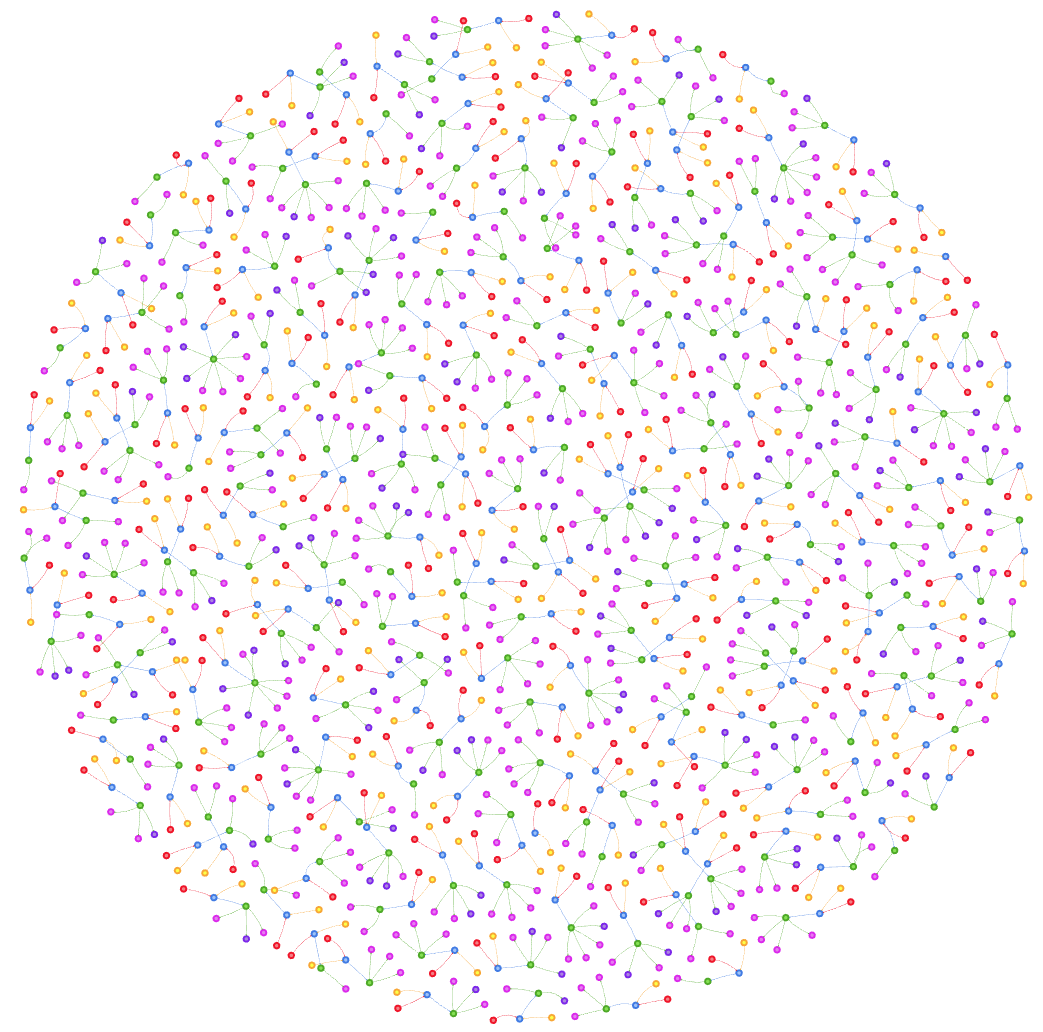
\includegraphics[width=0.7\columnwidth]{figures/g.V().png}
    \caption{A visualization of collected 209 collaboration patterns (CPs) as 209 knowledge graphs (KGs).}
    \label{fig:cps_all_visualized}
\end{subfigure}

\vspace{1em}

%--------------------------------------------
% Subfigure (b) - Example CP visualization
%--------------------------------------------
\begin{subfigure}[b]{\columnwidth}
    \centering
    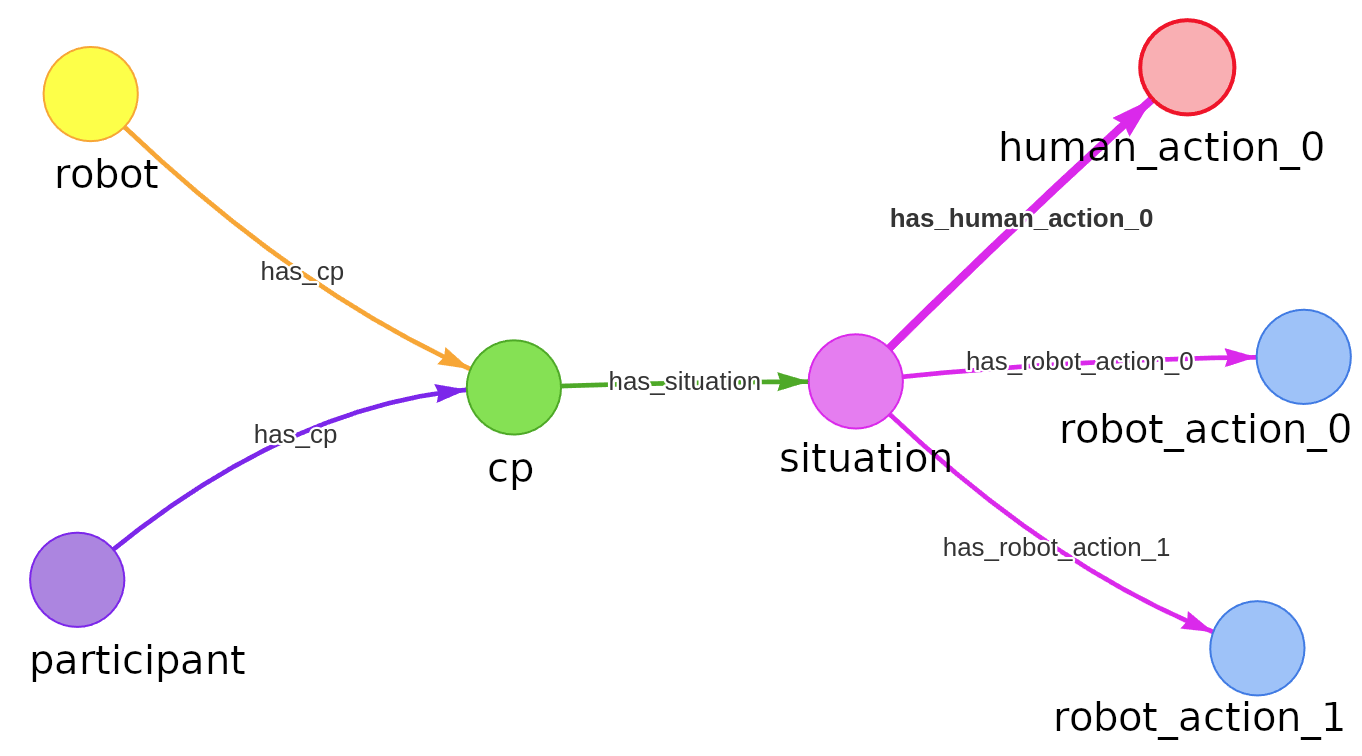
\includegraphics[width=0.75\columnwidth]{figures/cp_36.png}
    \caption{A visualization of an example CP. This knowledge graph (KG) has seven nodes: one \texttt{robot}, \texttt{participant}, \texttt{cp}, and \texttt{situation}, along with one \texttt{human\_action} and two \texttt{robot\_action} nodes. While all CPs share the same core structure, the number of \texttt{human\_action} and \texttt{robot\_action} nodes varies, as annotators define action sequences for the human and robot. A KG structure allows for this flexibility, handling dynamic node and edge counts, including varying number of \texttt{has\_human\_action} and \texttt{has\_robot\_action} edges.}
    \label{fig:cp_36_visualized}
\end{subfigure}

\caption{Visualizations of collaboration patterns (CPs) represented as knowledge graphs (KGs). (a) The entire set of 209 CPs. (b) An example CP illustrating its structural components.}
\label{fig:cp_visualization}
\end{figure}


\section{Methodology}
\label{sec:methodology}

\subsection{Ontology Engineering}
\label{sec:ontology}

Because CP graphs have variable topology, we represent them as property graphs rather than force‑fitting them into fixed‑length Euclidean vectors, thus retaining full relational context.

Our ontology defines six entity types: \texttt{robot}, \texttt{participant}, \texttt{cp}, \texttt{situation}, \texttt{robot\_action}, and \texttt{human\_action}. Each entity is represented as a node with associated properties. Relationships between entities are captured through four edge types: \texttt{has\_cp}, \texttt{has\_situation}, \texttt{has\_robot\_action}, and \texttt{has\_human\_action}, each of which can also store relevant properties. This structure provides a flexible and expressive representation of CPs, allowing detailed analysis of human-robot interactions.

From the previous studies, we have collected 209 CPs. Figure~\ref{fig:cp_visualization} visualizes them. We used the JanusGraph-Visualizer~\cite{janusgraph_2024}. 


Table~\ref{tab:cp_properties} lists the node properties of the example CP visualized in Figure~\ref{fig:cp_36_visualized}. The \texttt{cp} node properties ``time\_elapsed'', ``remaining\_rocks'', ``victim\_harm'', and ``success'', serve as round-level performance metrics. While not CP-specific, we assume that if the human-robot team performs well in a round, the CPs used contribute to that success.

\begin{table}[tb]
    \centering
    \renewcommand{\arraystretch}{1.2}
    \begin{tabular}{p{2.5cm} p{5.5cm}}
        \toprule
        \textbf{Type} & \textbf{Properties} \\
        \midrule
        \texttt{robot} &  \\
        \midrule
        \texttt{participant} & participant\_number: 4081 \\
        \midrule
        \texttt{cp} & time\_elapsed: 3000, \newline event\_time: ``2024-05-07T11:26:11'', \newline cp\_num: 36, \newline ticks\_lasted: 1917, \newline participant\_num: 4081, \newline remaining\_rocks: 32, \newline cp\_name: ``top brown'', \newline victim\_harm: 0, \newline success: false \newline round\_num: 6 \\
        \midrule
        \texttt{situation} & location: ``Top of rock pile'', \newline object: ``Brown rock'' \\
        \midrule
        \texttt{human\_action\_0} & location: ``Above rock pile'', \newline action: ``Stand still in \textless location\textgreater'' \\
        \midrule
        \texttt{robot\_action\_0} & location: ``Top of rock pile'', \newline object: ``Brown rock'', \newline action: ``Pick up \textless object\textgreater in \textless location\textgreater'' \\
        \midrule
        \texttt{robot\_action\_1} & location: ``\textless Right\textgreater side of field'', \newline object: ``Brown rock'', \newline action: ``Drop \textless object\textgreater in \textless location\textgreater'' \\
        \bottomrule
    \end{tabular}
    \caption{The node properties of the example CP.}
    \label{tab:cp_properties}
\end{table}

\subsection{Self-Supervised Learning on Graphs}
\label{sec:graph_learning}

Choosing a CP by raw score alone ignores the situational and action context that produced that score. A high-performing CP in one scenario may not generalize to others. To address this, we cluster CPs using self-supervised graph learning, capturing both performance and structural similarities. This enables us to identify the most representative and effective CPs for improved collaboration. 

Since our CPs are structured as KGs, we use a Relational Graph Convolutional Network (RGCN)~\cite{schlichtkrull2017modelingrelationaldatagraph} to learn meaningful representations. Unlike standard GNNs, RGCN incorporates edge types (e.g., \texttt{has\_cp}, \texttt{has\_human\_action}), which capture essential relational information. Through message passing, RGCN iteratively updates node features, allowing interactions between entities to shape their representations. To enable self-supervised learning, we perform node classification by adding a linear layer with softmax on top of the final RGCN layer. Each node belongs to a predefined class (e.g., \texttt{participant}, \texttt{situation}, \texttt{human\_action}), and the model learns to predict these labels. The message-passing mechanism ensures that gradients propagate beyond individual nodes, influencing their neighbors and refining the entire graph representation.

As shown in Table~\ref{tab:cp_properties}, node properties contain various features, requiring transformation into fixed-length vectors for RGCN compatibility. For \texttt{cp} nodes, we concatenate six numerical features (``time\_elapsed'', ``ticks\_lasted'', ``remaining\_rocks'', ``victim\_harm'', ``success'', and ``round\_num''), normalizing each by its maximum value to scale them between 0 and 1. For \texttt{situation}, \texttt{human\_action}, and \texttt{robot\_action} nodes, we concatenate string attributes into natural language sentences (e.g., \texttt{human\_action\_0} in the example would be ``Action: Stand still in \textless location\textgreater. Location: Above rock pile.'') and encode them using Sentence-BERT~\cite{reimers2019sentencebertsentenceembeddingsusing} to obtain numerical vector representations. Since the \texttt{cp} node vectors are shorter than the others, we apply a learnable projection matrix to transform them to the same dimensionality as the vectors for \texttt{situation}, \texttt{human\_action}, and \texttt{robot\_action} nodes.

We optimize RGCN using cross-entropy loss for node classification. Let \( f_{\theta} \) represent the entire model, including RGCN and the linear classifier. Given a CP (KG) \( \mathcal{G} \) with node features \( X \) and adjacency matrix \( A \), the predicted class distribution for a node \( v \) is:

\[
\hat{y}_v = \text{softmax}(f_{\theta}(\mathcal{G}, X, A)_v)
\]

where \( f_{\theta} \) processes the entire graph structure, and \( \theta \) includes all trainable parameters. The loss function is:

\[
\mathcal{L} = - \mathbb{E}_{(v, c) \sim \mathcal{D}_\text{train}} \left[ \log \hat{y}_{v, c} \right]
\]

where \(\mathcal{D}_\text{train}\) represents the empirical distribution of training samples, and \(C\) is the number of node classes. 

The message-passing mechanism propagates updates across the graph, refining node representations based on their connectivity. Consecutive human actions (e.g., \texttt{human\_action\_0}, \texttt{human\_action\_1}, \texttt{human\_action\_2}) and robot actions (e.g., \texttt{robot\_action\_0} to \texttt{robot\_action\_4}) are treated as distinct classes, as they represent different stages within an action sequence. Thus, we set \(C = 10\). See Figure~\ref{fig:rgcn} for a visualization of one forward pass of the RGCN-based neural network.

\begin{figure}[tb]
\centering
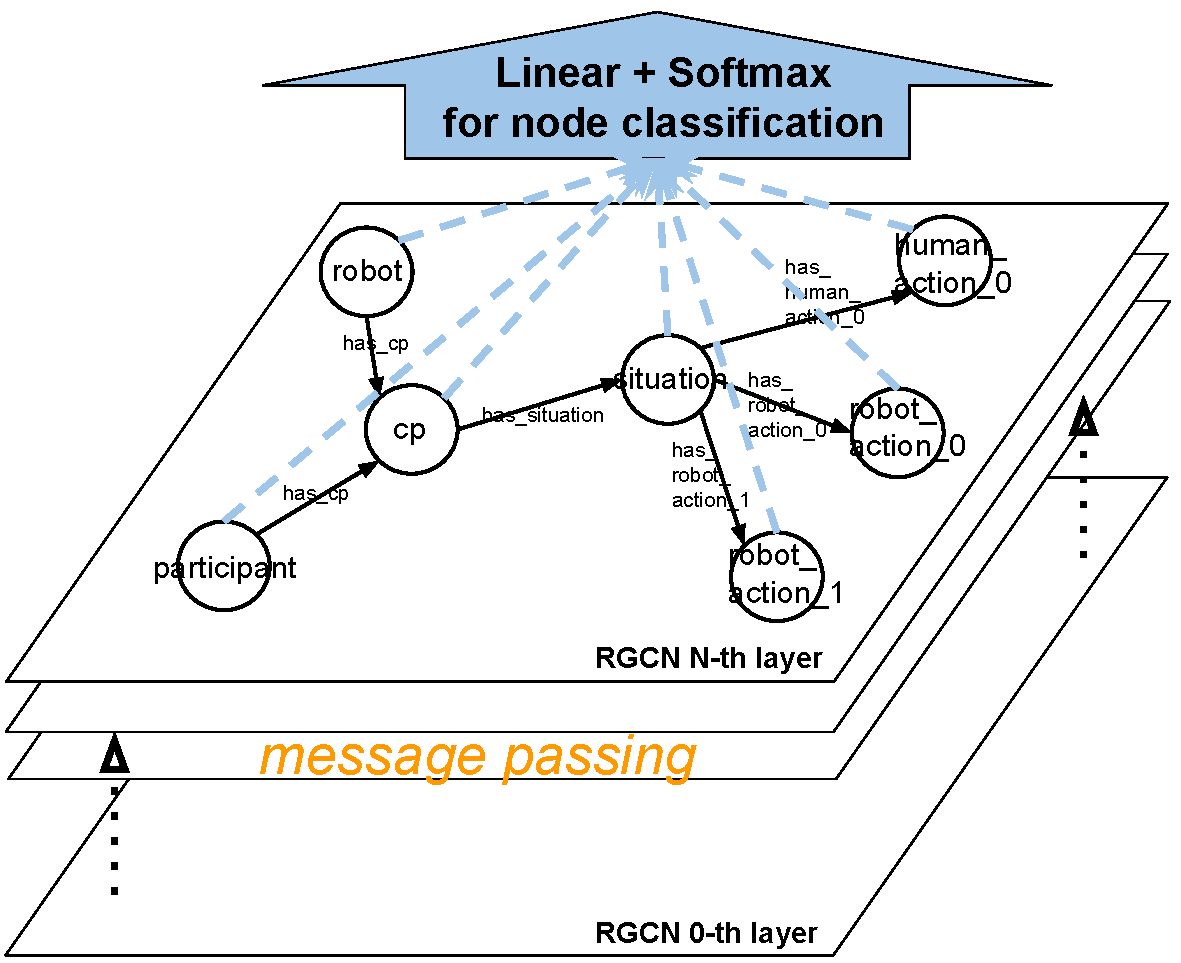
\includegraphics[width=\columnwidth]{figures/rgcn-co-learning.pdf}
\caption{A forward pass of the RGCN-based neural network. The last layer (Linear + Softmax) outputs the categorical distributions which are combined with the ground truths to compute the cross entropy loss.}
\label{fig:rgcn}
\end{figure}

After the self-supervised learning phase, we use the learned graph representations to cluster the CPs. From these clusters, we select the most representative CP, which we then use to initialize the robot’s memory. This enables the robot to start with the ``best'' episodic memory, providing it with structured prior knowledge. We then conduct human-robot interaction experiments in the same MATRX collaborative environment to evaluate the impact of this memory augmentation on task performance metrics.

\section{Experiments}
\label{sec:experiments}

The two‑layer RGCN (128,874 parameters, ReLU activations) trained for 2,000 epochs on all 209 CP graphs in a single 30s CPU run; code and hyper‑parameters are in the supplementary material, along with a recorded game play and raw data. See Figure~\ref{fig:training} for the training loss, which steadily decreases over epochs, while the accuracy increases, indicating effective learning and convergence of the model.

\begin{figure}[tb]
\centering
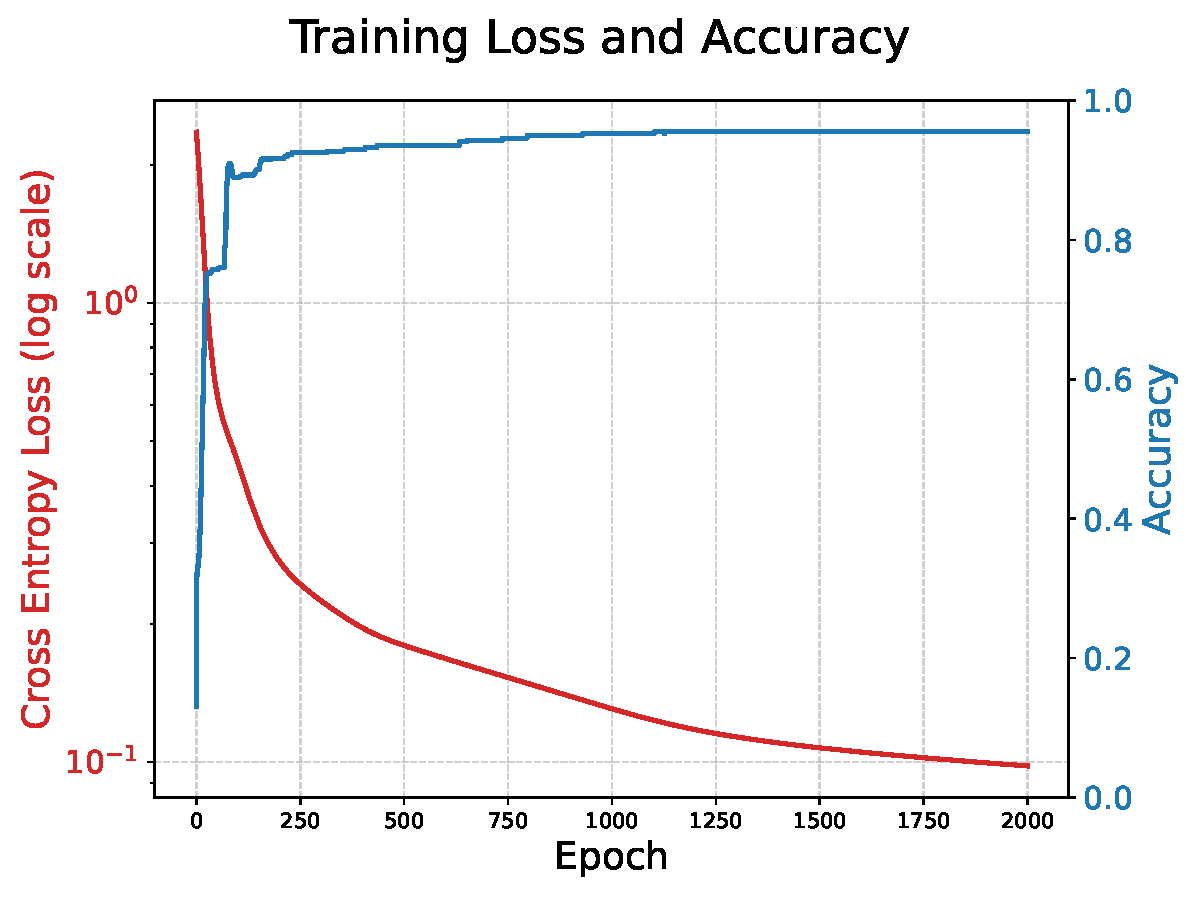
\includegraphics[width=\columnwidth]{figures/Training_Loss_and_Accuracy.pdf}
\caption{Cross entropy loss and accuracy of the training data. After 2,000 epochs, the loss dropped to 0.0948 while the accuracy went up to 95.5\%.}
\label{fig:training}
\end{figure}

After training, we obtain the final vector representation of each CP by averaging the node representations (before the classification layer) within each graph. We then apply the K-means clustering algorithm to group CPs based on Euclidean distance. Figure~\ref{fig:cluster} illustrates the clusters before and after training, with t-SNE~\cite{NIPS2002_6150ccc6} used for 2D visualization. It can be seen that the self‑supervised GNN learns the meaningful representations to cluster CPs. The number of CPs in the clusters are 62, 38, 36, 30, and 43, respectively.

\begin{figure}[tb]
\centering

\begin{subfigure}[b]{\columnwidth}
    \centering
    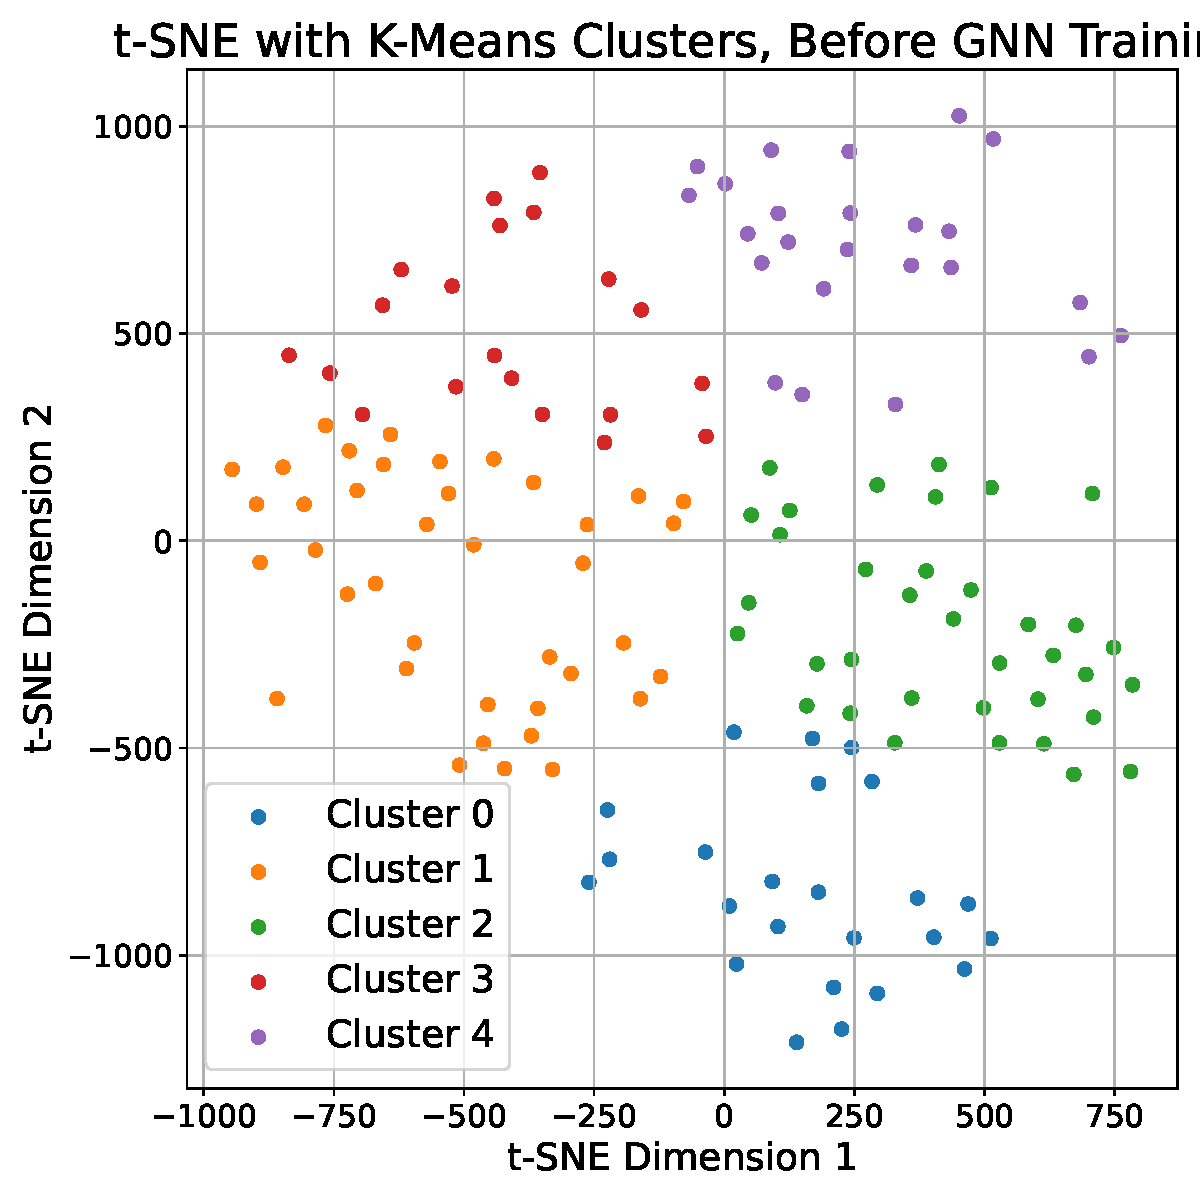
\includegraphics[width=0.66\columnwidth]{figures/t-SNE with K-Means Clusters, Before GNN Training.pdf}
    \caption{5 clusters of CPs before training. Since there are not yet GNN-based vector representations for the CPs, we used the \texttt{cp} node features as vectors.}
    \label{fig:cluster_before_training}
\end{subfigure}

\vspace{1em}

\begin{subfigure}[b]{\columnwidth}
    \centering
    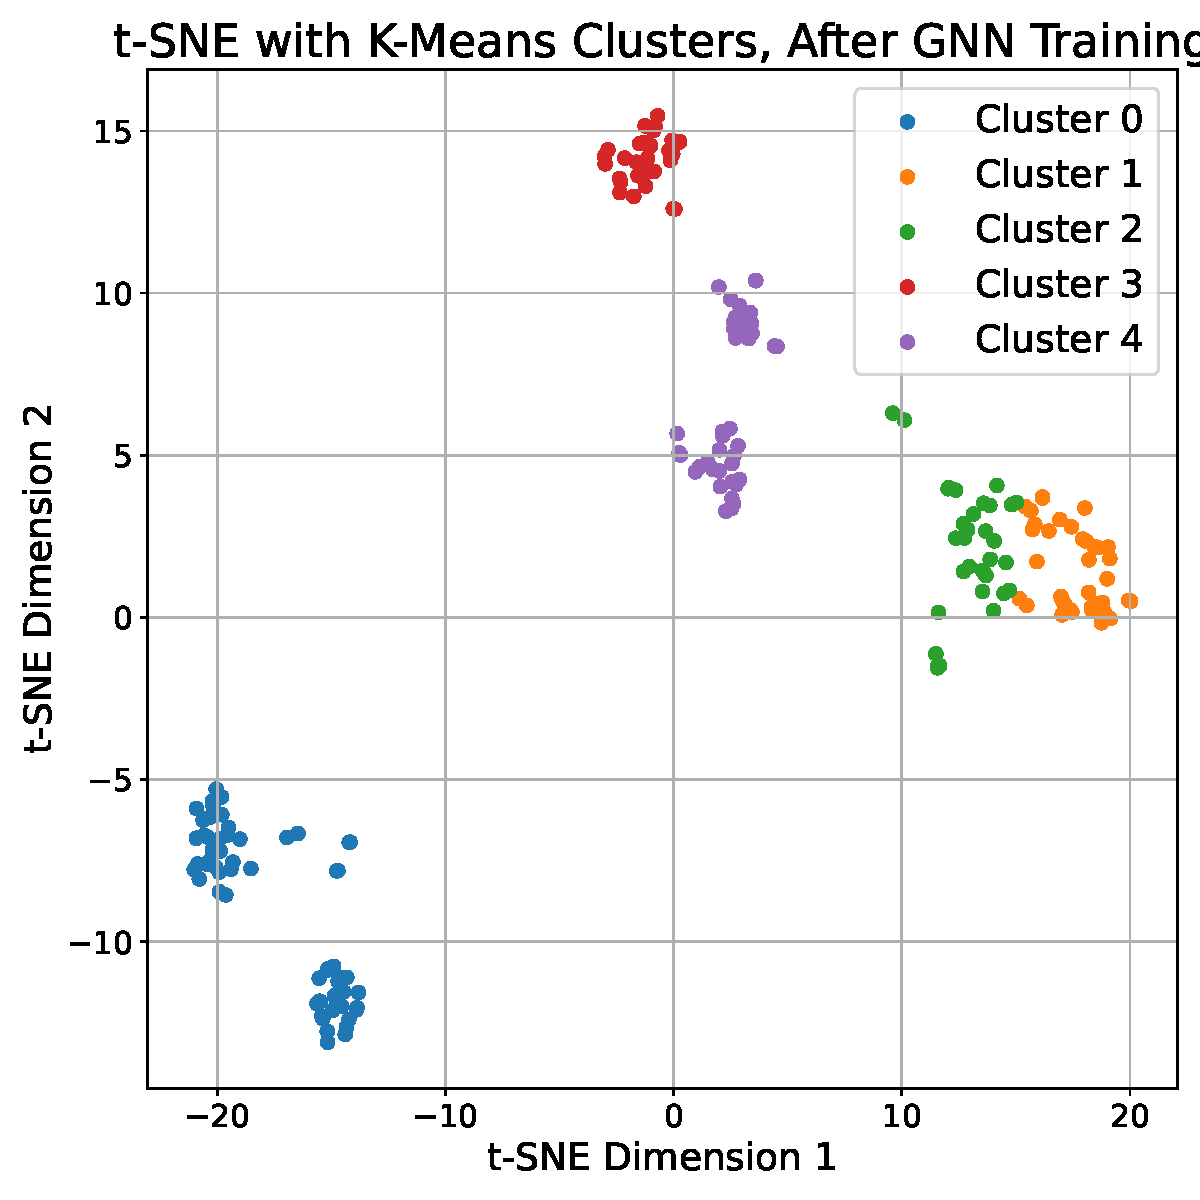
\includegraphics[width=0.66\columnwidth]{figures/t-SNE with K-Means Clusters, After GNN Training.pdf}
    \caption{5 clusters of CPs after training. The vectors used here are the means of the last RGCN layer node representations.}
    \label{fig:cluster_after_training}
\end{subfigure}

\caption{K-means clustering results before and after training, visualized using t-distributed stochastic neighbor embedding (t-SNE) to map high-dimensional vectors into 2D space. $K=5$ was chosen.}
\label{fig:cluster}
\end{figure}


Table~\ref{tab:cluster_stats} presents the performance metrics for each cluster. Notably, Cluster 1 exhibits a higher success rate, suggesting that participants using CPs from this cluster were more likely to rescue the victim. While the other metrics remain important, we emphasize success rate since saving the victim is considered the most critical outcome.

\begin{table}[tb]
    \centering
    \renewcommand{\arraystretch}{1.2}
    \resizebox{\columnwidth}{!}{ % Rescale table
    \begin{tabular}{lcccc}
        \toprule
        \textbf{Cluster} & \makecell{\textbf{Time} \\ \textbf{Elapsed}} & \makecell{\textbf{Remaining} \\ \textbf{Rocks}} & \makecell{\textbf{Victim} \\ \textbf{Harm}} & \makecell{\textbf{Sucess} \\ \textbf{Rate}} \\
        \midrule
        Cluster 0 & 2716 (+120) & 16 (+1.0) & 291 (-14) & 24\% (-3\%) \\
        Cluster 1 & 2133 (-462) & 11 (-3.9) & 318 (+11) & 42\% (+15\%) \\
        Cluster 2 & 2607 (+12) & 11 (-3.2) & 311 (+4) & 36\% (+9\%) \\
        Cluster 3 & 2869 (+273) & 18 (+3.9) & 246 (-60) & 17\% (-11\%) \\
        Cluster 4 & 2629 (+33) & 16 (+1.9) & 355 (+49) & 19\% (-9\%) \\
        \bottomrule
    \end{tabular}
    }
    \caption{Cluster statistics (higher is better for success rate and lower is better for the others.), with differences from the mean in parentheses.}
    \label{tab:cluster_stats}
\end{table}

Table~\ref{tab:cluster_edges} presents the edge types and their frequencies for the CPs in each cluster. Notably, the action edges in Cluster 1 are simpler than those in other clusters, as it contains fewer distinct action types. Of the 78 total edges across all CPs in Cluster 1, the majority involve two consecutive robot actions. This suggests that Cluster 1 not only represents a simpler interaction pattern but also grants greater autonomy to the robot. While robot actions are typically conditioned on human actions, the lower presence of human action edges in this cluster indicates that the robot's behavior is less dependent on human input.

\begin{table}[tb]
    \centering
    \renewcommand{\arraystretch}{1.2}
    \setlength{\tabcolsep}{8pt}
    \begin{tabular}{llc}
        \toprule
        \textbf{Cluster} & \textbf{Edge label} & \textbf{Count (\%)} \\
        \midrule
        \multirow{7}{*}{Cluster 0} 
        & has\_robot\_action\_0 & 62 (55.86\%) \\
        & has\_human\_action\_0 & 30 (27.03\%) \\
        & has\_human\_action\_1 & 8 (7.21\%) \\
        & has\_robot\_action\_2 & 3 (2.70\%) \\
        & has\_robot\_action\_3 & 3 (2.70\%) \\
        & has\_robot\_action\_4 & 3 (2.70\%) \\
        & has\_human\_action\_2 & 2 (1.80\%) \\
        \midrule
        \multirow{3}{*}{Cluster 1} 
        & has\_robot\_action\_1 & 38 (48.72\%) \\
        & has\_robot\_action\_0 & 38 (48.72\%) \\
        & has\_robot\_action\_2 & 2 (2.56\%) \\
        \midrule
        \multirow{6}{*}{Cluster 2} 
        & has\_robot\_action\_1 & 36 (31.30\%) \\
        & has\_robot\_action\_0 & 36 (31.30\%) \\
        & has\_robot\_action\_2 & 31 (26.96\%) \\
        & has\_robot\_action\_3 & 7 (6.09\%) \\
        & has\_human\_action\_1 & 4 (3.48\%) \\
        & has\_human\_action\_2 & 1 (0.87\%) \\
        \midrule
        \multirow{4}{*}{Cluster 3} 
        & has\_human\_action\_0 & 30 (38.46\%) \\
        & has\_robot\_action\_1 & 30 (38.46\%) \\
        & has\_robot\_action\_2 & 16 (20.51\%) \\
        & has\_robot\_action\_3 & 2 (2.56\%) \\
        \midrule
        \multirow{7}{*}{Cluster 4} 
        & has\_human\_action\_0 & 43 (26.22\%) \\
        & has\_robot\_action\_1 & 43 (26.22\%) \\
        & has\_robot\_action\_0 & 42 (25.61\%) \\
        & has\_human\_action\_1 & 20 (12.20\%) \\
        & has\_robot\_action\_2 & 7 (4.27\%) \\
        & has\_robot\_action\_3 & 7 (4.27\%) \\
        & has\_human\_action\_2 & 2 (1.22\%) \\
        \bottomrule
    \end{tabular}
    \caption{Edge label distributions across clusters.}
    \label{tab:cluster_edges}
\end{table}


Considering both performance and structural simplicity, we identified Cluster 1 as the most meaningful set of CPs. It represents a minimal yet effective CP, where the robot operates with greater autonomy while maintaining efficiency. We selected the CP closest to the cluster center (by Euclidean distance) as our final choice, as it best represents the defining characteristics of Cluster 1 and serves as the most typical example of its CP.

Table~\ref{tab:final_cp} presents the final selected CP. Notably, this CP consists of only two consecutive robot actions without any human actions. This suggests that, in this scenario, the robot operates independently, executing its tasks without relying on human input. Compared to other CPs that typically involve human actions, this CP grants the robot greater autonomy in decision-making and task execution. Specifically, this CP directs the robot to move large rocks near the victim. Since only the robot can handle large rocks, this pattern effectively delegates the heavy lifting to the robot while allowing the human to focus on other tasks as they see fit.

\begin{table}[h]
    \centering
    \renewcommand{\arraystretch}{1.2}
    \setlength{\tabcolsep}{5pt}
    \begin{tabular}{lp{5cm}}
        \toprule
        \textbf{Type} & \textbf{Details} \\
        \midrule
        \texttt{situation} & Location: ``Top of rock pile'' \newline
                   Object: ``Large rock'' \\
        \midrule
        \texttt{robot\_action\_0} & Location: ``Top of rock pile'' \newline
                         Object: ``Large rock'' \newline
                         Action: ``Pick up \textless object\textgreater{} in \textless location\textgreater{}'' \\
        \midrule
        \texttt{robot\_action\_1} & Location: ``\textless Right\textgreater{} side of field'' \newline
                         Object: ``Large rock'' \newline
                         Action: ``Drop \textless object\textgreater{} in \textless location\textgreater{}'' \\
        \bottomrule
    \end{tabular}
    \caption{The final selected collaboration pattern (CP).}
    \label{tab:final_cp}
\end{table}

We initialize the robot's memory with the final CP and conduct the MATRX USAR experiment under the same conditions as the previous study, with the only difference being the inclusion of the preloaded memory. We recruited 20 student participants from our university. All experiments were conducted online.\footnote{The experiment involving human participants was approved by our university's ethics committee (ID anonymized).}

\begin{table*}[tb]
    \centering
    \renewcommand{\arraystretch}{1.2}
    \setlength{\tabcolsep}{6pt}
    \resizebox{\textwidth}{!}{ % Ensure table fits within the page width
    \begin{tabular}{c|cc|cc|cc|cc}
    \toprule
    \multirow{2}{*}{Round} 
    & \multicolumn{2}{c|}{\textbf{Time Elapsed}} 
    & \multicolumn{2}{c|}{\textbf{Remaining Rocks}} 
    & \multicolumn{2}{c|}{\textbf{Victim Harm}} 
    & \multicolumn{2}{c}{\textbf{Success Rate}} \\
    & \textbf{\makecell{W/o Memory \\ Initialized}} & \textbf{\makecell{With Memory \\ Initialized}} 
    & \textbf{\makecell{W/o Memory \\ Initialized}} & \textbf{\makecell{With Memory \\ Initialized}} 
    & \textbf{\makecell{W/o Memory \\ Initialized}} & \textbf{\makecell{With Memory \\ Initialized}} 
    & \textbf{\makecell{W/o Memory \\ Initialized}} & \textbf{\makecell{With Memory \\ Initialized}} \\
    \midrule
    1  & 3000 (0)   & 2458 (626)  & 18.2 (6.0)   & 5.8 (8.0)   & 733 (512)  & 160 (320)  & 0.0\% (0.0\%)    & 55.0\% (51.0\%)  \\
    2  & 2677 (604) & 2304 (644)  & 14.5 (13.3)  & 5.3 (8.1)   & 324 (387)  & 255 (349)  & 28.5\% (46.3\%)  & 65.0\% (48.9\%)  \\
    3  & 2410 (707) & 2192 (732)  & 10.4 (13.7)  & 3.5 (7.3)   & 257 (457)  & 465 (589)  & 52.4\% (51.1\%)  & 75.0\% (44.4\%)  \\
    4  & 2475 (699) & 2150 (672)  & 7.9 (9.5)    & 3.5 (7.0)   & 286 (408)  & 160 (201)  & 47.6\% (51.2\%)  & 75.0\% (44.4\%)  \\
    5  & 2493 (722) & 2300 (720)  & 15.9 (12.0)  & 12.0 (9.5)  & 457 (383)  & 470 (508)  & 23.8\% (43.6\%)  & 30.0\% (47.0\%)  \\
    6  & 2590 (630) & 2593 (545)  & 19.0 (9.6)   & 14.0 (7.7)  & 476 (648)  & 520 (393)  & 4.7\% (21.8\%)   & 15.0\% (36.6\%)  \\
    7  & 2503 (555) & 1994 (784)  & 15.5 (11.9)  & 17.1 (6.9)  & 310 (319)  & 880 (635)  & 23.8\% (43.6\%)  & 5.0\% (22.4\%)   \\
    8  & 2558 (545) & 2448 (660)  & 14.5 (11.4)  & 12.5 (6.9)  & 535 (701)  & 1190 (679) & 25.0\% (44.4\%)  & 10.0\% (30.8\%)  \\
    \midrule
    \textbf{Overall} 
    & 2588 (613)  & \textbf{2305 (686)}  
    & 14.5 (11.4) & \textbf{9.2 (9.1)}  
    & \textbf{422 (504)}   & 513 (583)  
    & 25.7\% (43.9\%)  & \textbf{41.3\% (49.4\%)}  \\
    \bottomrule
    \end{tabular}
    }
    \caption{Comparison of the robot without initialized memory and the robot with initialized memory. 
    Values are presented as \textit{Average (std)}, where standard deviation is in parentheses. 
    Success rate is reported as a percentage (\%), where higher is better; lower is better for the other metrics. 
    Both the robot without memory and the robot with initialized memory were evaluated using 20 samples (participants) each. Better values for each metric are shown in \textbf{bold}.}
    \label{tab:comparison} 
\end{table*}

Table~\ref{tab:comparison} shows that the robot with initialized memory consistently outperforms the one without it, except in ``victim\_harm,'' likely due to accidental rock falls when removing large rocks. Statistical analysis confirms this improvement is significant: with $n = 8 \times 20 = 160$ observations per group, the success rate increased from 25.7\% to 41.3\% (a 60.7\% relative improvement), with $t(318) = 2.986$, $p = 0.0015$ (one-tailed), and Cohen's $d = 0.334$. The 95\% confidence interval [5.3\%, 25.9\%] excludes zero, confirming the reliability of our findings. Notably, the most significant improvement occurs in Round 1, where participants are still unfamiliar with the environment. Since the robot begins with prior knowledge from past interactions, it can immediately engage in effective collaboration, providing a smoother start for the human-robot team.

Interestingly, the selected CP (Table~\ref{tab:final_cp}) does not reference the ``Brown rock,'' which only appears in later rounds (Rounds 5–8). Despite this, the robot with initialized memory continues to facilitate better performance in most of the rounds, except 7 and 8. This suggests that the chosen CP captures a generally effective collaboration strategy, enabling the robot to adapt even in scenarios it has not explicitly encountered before.

\section{Related Work}
\label{sec:related_work}

Our work builds on several research strands, including human-like memory in agents, KG representations for complex relational data, graph neural networks for structured learning, and human-robot collaboration in challenging environments such as urban search and rescue (USAR). In this section, we discuss these lines of research and position our contribution in relation to existing approaches.

Our work is inspired by the concept of agents' episodic memory, where past experiences are stored and reactivated to guide future actions. Early approaches, drawing on cognitive science, used symbolic and rule-based systems to mimic human memory functions in agents. More recent methods, such as those by Parisotto et al.~\cite{pmlr-v70-pritzel17a} and Rebuffi et al.~\cite{chaudhry2019efficientlifelonglearningagem}, employ deep learning to capture and encode complex interaction patterns, enabling agents to both recall and generalize from previous experiences. We extend these ideas by representing episodic memories as KGs, providing a structured format that captures performance metrics and contextual details of human-agent collaborations, thereby facilitating more effective retrieval and application of prior experiences in challenging scenarios.

Kim et al.~\cite{https://doi.org/10.48550/arxiv.2204.01611,Kim_Cochez_Francois-Lavet_Neerincx_Vossen_2023} adopted a cognitive science-inspired approach to develop a human-like memory system. Their agents incorporate both episodic and semantic memory components. In their framework, episodic memory captures the agent's direct experiences, while semantic memory encompasses general factual knowledge—information that can be acquired through learning or provided by human experts.

Self-supervised learning is central to modern large language models like BERT~\cite{DBLP:journals/corr/abs-1810-04805} and GPT-3~\cite{DBLP:journals/corr/abs-2005-14165}, which capture rich contextual information from unlabeled data by reconstructing or predicting missing parts (e.g., via masked language modeling or next-token prediction). Similarly, self-supervised techniques in graph neural networks enable the extraction of meaningful embeddings from inherently unlabeled node data. These learned representations, which capture structural and relational nuances, can then be leveraged for downstream tasks such as clustering. In our work, we use self-supervised graph learning to derive robust representations of episodic memory KGs, facilitating efficient clustering of CPs.

Collaborative learning in human-robot teams has emerged as a pivotal factor for enabling mutual adaptation and shared understanding in dynamic task environments. Baxter et al.~\cite{Baxter2017RobotEP} demonstrated that personalized interactions between robots and human learners can significantly enhance educational outcomes, setting the stage for further exploration into adaptive team behaviors. Building on this, Belpaeme et al.~\cite{Belpaeme2018} provided comprehensive guidelines for designing social robots that effectively serve as second language tutors, emphasizing the importance of interactive, adaptive strategies. Complementing these efforts, Nikolaidis et al.~\cite{Nikolaidis} investigated mutual adaptation in collaborative tasks, offering experimental evidence that both humans and robots benefit from continuous reciprocal learning. Moreover, Holstein et al.~\cite{Holstein} introduced a conceptual framework for human-AI hybrid adaptivity in educational settings, highlighting how effective communication and adaptive strategies can jointly drive collaborative learning. These studies collectively underscore the potential of leveraging mutual adaptation to foster robust and resilient human-robot partnerships.

Collaborative work has further enriched our understanding of human-robot co-learning. For instance, Shafti et al.~\cite{DBLP:journals/corr/abs-2003-01156} demonstrated effective human-robot collaboration through reinforcement learning in real-world scenarios, while Wenskovitch et al.~\cite{WenskovitchInteractiveAD} addressed the challenge of transparency in interactive AI systems, emphasizing the need for interpretable decision-making in collaborative settings. Moreover, Gao et al.~\cite{gao} explored personalized human-robot co-adaptation in instructional environments, highlighting how tailored interaction strategies can enhance mutual learning. These studies complement the aforementioned works by providing diverse perspectives on designing adaptive, communicative, and transparent systems for robust human-robot collaboration.

Recent work by van Zoelen et al.~\cite{10.1145/3434074.3446354,vanZoelen2021,vanZoelen2022} systematically identified recurring interaction patterns in human-robot co-adaptation using the MATRX USAR environment. Their study distinguishes between stable situations and sudden adaptations, offering a behavioral framework that captures the dynamics of mutual adaptation in team settings. These insights underscore the context-dependent nature of co-learning and provide a valuable foundation for designing systems that support effective human-robot interactions. Building on this work, our approach integrates KG-based representations of episodic memory with self-supervised graph learning, enabling efficient clustering and retrieval of these interaction patterns to enhance team-level performance in dynamic environments.


\section{Conclusion}
\label{sec:conclusion}


We showed that initializing a USAR robot with a single collaboration pattern stored as a knowledge‑graph episodic memory, learned by self‑supervised relational GNNs, can boost human–robot teamwork. In 160 MATRX trials the seeded robot raised victim‑rescue success from 25.7\% to 41.3\% and cut average task time by 283s. However, the study also comes with some limitations. It was limited to simulation with 20 student participants, one CP drawn from the best cluster, and a domain‑specific ontology; budget constraints precluded testing other cluster exemplars, and victim‑harm sometimes increased when the robot moved heavy debris. Future work will pursue online growth / pruning of the episodic memory and transfer to other collaborative domains.


\bibliography{aaai2026}

% Check whether the conference requires a reproducibility checklist to be included in the paper.
% If so, you can uncomment the following line and ajust the path to include it.
\makeatletter
\@ifundefined{isChecklistMainFile}{
  % We are compiling a standalone document
  \newif\ifreproStandalone
  \reproStandalonetrue
}{
  % We are being \input into the main paper
  \newif\ifreproStandalone
  \reproStandalonefalse
}
\makeatother

\ifreproStandalone
\documentclass[letterpaper]{article}
\usepackage[submission]{aaai2026}
\setlength{\pdfpagewidth}{8.5in}
\setlength{\pdfpageheight}{11in}
\usepackage{times}
\usepackage{helvet}
\usepackage{courier}
\usepackage{xcolor}
\frenchspacing

\begin{document}
\fi
\setlength{\leftmargini}{20pt}
\makeatletter\def\@listi{\leftmargin\leftmargini \topsep .5em \parsep .5em \itemsep .5em}
\def\@listii{\leftmargin\leftmarginii \labelwidth\leftmarginii \advance\labelwidth-\labelsep \topsep .4em \parsep .4em \itemsep .4em}
\def\@listiii{\leftmargin\leftmarginiii \labelwidth\leftmarginiii \advance\labelwidth-\labelsep \topsep .4em \parsep .4em \itemsep .4em}\makeatother

\setcounter{secnumdepth}{0}
\renewcommand\thesubsection{\arabic{subsection}}
\renewcommand\labelenumi{\thesubsection.\arabic{enumi}}

\newcounter{checksubsection}
\newcounter{checkitem}[checksubsection]

\newcommand{\checksubsection}[1]{%
  \refstepcounter{checksubsection}%
  \paragraph{\arabic{checksubsection}. #1}%
  \setcounter{checkitem}{0}%
}

\newcommand{\checkitem}{%
  \refstepcounter{checkitem}%
  \item[\arabic{checksubsection}.\arabic{checkitem}.]%
}
\newcommand{\question}[2]{\normalcolor\checkitem #1 #2 \color{blue}}
\newcommand{\ifyespoints}[1]{\makebox[0pt][l]{\hspace{-15pt}\normalcolor #1}}

\section*{Reproducibility Checklist}

\vspace{1em}
\hrule
\vspace{1em}

\textbf{Instructions for Authors:}

This document outlines key aspects for assessing reproducibility. Please provide your input by editing this \texttt{.tex} file directly.

For each question (that applies), replace the ``Type your response here'' text with your answer.

\vspace{1em}
\noindent
\textbf{Example:} If a question appears as
%
\begin{center}
\noindent
\begin{minipage}{.9\linewidth}
\ttfamily\raggedright
\string\question \{Proofs of all novel claims are included\} \{(yes/partial/no)\} \\
Type your response here
\end{minipage}
\end{center}
you would change it to:
\begin{center}
\noindent
\begin{minipage}{.9\linewidth}
\ttfamily\raggedright
\string\question \{Proofs of all novel claims are included\} \{(yes/partial/no)\} \\
yes
\end{minipage}
\end{center}
%
Please make sure to:
\begin{itemize}\setlength{\itemsep}{.1em}
\item Replace ONLY the ``Type your response here'' text and nothing else.
\item Use one of the options listed for that question (e.g., \textbf{yes}, \textbf{no}, \textbf{partial}, or \textbf{NA}).
\item \textbf{Not} modify any other part of the \texttt{\string\question} command or any other lines in this document.\\
\end{itemize}

You can \texttt{\string\input} this .tex file right before \texttt{\string\end\{document\}} of your main file or compile it as a stand-alone document. Check the instructions on your conference's website to see if you will be asked to provide this checklist with your paper or separately.

\vspace{1em}
\hrule
\vspace{1em}

% The questions start here

\checksubsection{General Paper Structure}
\begin{itemize}

\question{Includes a conceptual outline and/or pseudocode description of AI methods introduced}{(yes/partial/no/NA)}
partial

\question{Clearly delineates statements that are opinions, hypothesis, and speculation from objective facts and results}{(yes/no)}
yes

\question{Provides well-marked pedagogical references for less-familiar readers to gain background necessary to replicate the paper}{(yes/no)}
yes

\end{itemize}
\checksubsection{Theoretical Contributions}
\begin{itemize}

\question{Does this paper make theoretical contributions?}{(yes/no)}
no

	% \ifyespoints{\vspace{1.2em}If yes, please address the following points:}
 %        \begin{itemize}
	
	% \question{All assumptions and restrictions are stated clearly and formally}{(yes/partial/no)}
	% Type your response here

	% \question{All novel claims are stated formally (e.g., in theorem statements)}{(yes/partial/no)}
	% Type your response here

	% \question{Proofs of all novel claims are included}{(yes/partial/no)}
	% Type your response here

	% \question{Proof sketches or intuitions are given for complex and/or novel results}{(yes/partial/no)}
	% Type your response here

	% \question{Appropriate citations to theoretical tools used are given}{(yes/partial/no)}
	% Type your response here

	% \question{All theoretical claims are demonstrated empirically to hold}{(yes/partial/no/NA)}
	% Type your response here

	% \question{All experimental code used to eliminate or disprove claims is included}{(yes/no/NA)}
	% Type your response here
	
	% \end{itemize}
\end{itemize}

\checksubsection{Dataset Usage}
\begin{itemize}

\question{Does this paper rely on one or more datasets?}{(yes/no)}
yes

\ifyespoints{If yes, please address the following points:}
\begin{itemize}

	\question{A motivation is given for why the experiments are conducted on the selected datasets}{(yes/partial/no/NA)}
	yes

	\question{All novel datasets introduced in this paper are included in a data appendix}{(yes/partial/no/NA)}
	yes

	\question{All novel datasets introduced in this paper will be made publicly available upon publication of the paper with a license that allows free usage for research purposes}{(yes/partial/no/NA)}
	yes

	\question{All datasets drawn from the existing literature (potentially including authors' own previously published work) are accompanied by appropriate citations}{(yes/no/NA)}
	yes

	\question{All datasets drawn from the existing literature (potentially including authors' own previously published work) are publicly available}{(yes/partial/no/NA)}
	partial

	\question{All datasets that are not publicly available are described in detail, with explanation why publicly available alternatives are not scientifically satisficing}{(yes/partial/no/NA)}
	partial

\end{itemize}
\end{itemize}

\checksubsection{Computational Experiments}
\begin{itemize}

\question{Does this paper include computational experiments?}{(yes/no)}
yes

\ifyespoints{If yes, please address the following points:}
\begin{itemize}

	\question{This paper states the number and range of values tried per (hyper-) parameter during development of the paper, along with the criterion used for selecting the final parameter setting}{(yes/partial/no/NA)}
	yes

	\question{Any code required for pre-processing data is included in the appendix}{(yes/partial/no)}
	yes

	\question{All source code required for conducting and analyzing the experiments is included in a code appendix}{(yes/partial/no)}
	yes

	\question{All source code required for conducting and analyzing the experiments will be made publicly available upon publication of the paper with a license that allows free usage for research purposes}{(yes/partial/no)}
	yes
        
	\question{All source code implementing new methods have comments detailing the implementation, with references to the paper where each step comes from}{(yes/partial/no)}
	yes

	\question{If an algorithm depends on randomness, then the method used for setting seeds is described in a way sufficient to allow replication of results}{(yes/partial/no/NA)}
	partial

	\question{This paper specifies the computing infrastructure used for running experiments (hardware and software), including GPU/CPU models; amount of memory; operating system; names and versions of relevant software libraries and frameworks}{(yes/partial/no)}
	yes

	\question{This paper formally describes evaluation metrics used and explains the motivation for choosing these metrics}{(yes/partial/no)}
	yes

	\question{This paper states the number of algorithm runs used to compute each reported result}{(yes/no)}
	partial

	\question{Analysis of experiments goes beyond single-dimensional summaries of performance (e.g., average; median) to include measures of variation, confidence, or other distributional information}{(yes/no)}
	yes

	\question{The significance of any improvement or decrease in performance is judged using appropriate statistical tests (e.g., Wilcoxon signed-rank)}{(yes/partial/no)}
	yes

	\question{This paper lists all final (hyper-)parameters used for each model/algorithm in the paper’s experiments}{(yes/partial/no/NA)}
	yes


\end{itemize}
\end{itemize}
\ifreproStandalone
\end{document}
\fi


\clearpage

\section{Reviews}

\subsection{Review 1}

\subsubsection*{Title}
Have some questions about details

\subsubsection*{Review}
\textbf{Summary of paper -}

This paper proposes to augment memory to a robot in a human robot collborative setting, and the paper shows a success rate as well as time decrease in task completion with such a memory augmented robot. The paper used an episodic memory and selects most representative memories using a K-Means clustering based approach on the learnt graph features, which is contucted using standard KG methods.

\textbf{Some questions/suggestions about the details -}
\begin{enumerate}
\item How were the \textbf{number of clusters} for the K Means clustering of the average representation of the penultimate layer chosen? Since this is a hyperparameter the work could show how the results are sensitive to the choice of this hyperparameter.
\item What exactly is the \textbf{policy} that is being learnt here by the robot for human robot collaboration? Is it rule based policy? Or is it a parametrized policy? Or is it just the case that there are some pre-programmed behaviors that the robot and human can do which are described in text format, and there is a communication channel (i.e. the text interface)? The state and action space are a little unlcear to me, i.e. the markov decision process that describes environment could be made clearer. Unfamiliary with the MATRX environment could be the root cause of this question.
\item How exactly is the \textbf{"robot memory"} being initalized, i.e what is a robot memory? What is the data structure that is being used for this memory and how is this being used while the robot is executing its policy? This could be made clearer in this work.
\item A minor point about \textbf{terminology} - the representation learning of the features of the GNN is being referred to as self supervised learning, but rather it is more like representation learning using a supervised classification loss of nodes (this isn't self supervised learning to be strict in the terminology, since some kind of labels are being used)
\item What are the \textbf{episodes} that are being used, is it just the previous interaction history with the humans? In this case it could be made clearer what is the size of this memory, since it is inherently unfair to a robot which uses no memory during performance comparsion, since the memory-based robot inherently has more computational power.
\item The work should cite a reference to a literature review on continual learning which is widely used in machine learning, espicially episodic-memory based CL which is a major continual learning paradigm.
\end{enumerate}

\textbf{Summary of review -}

The major thing that the work can improve on is adding some details of to the first part, i.e. the task and environment description. The description of the GNN construction and clustering is mostly clear. It is outlined in the above suggestion section. The paper is above acceptance threshold, but if subsequent versions could address the above details, it will make the case stronger. Reviewer willing to raise score if above details are addressed.

\subsubsection*{Rating}
6: Marginally above acceptance threshold

\subsubsection*{Confidence}
4: The reviewer is confident but not absolutely certain that the evaluation is correct

\subsection{Review 2}

\subsubsection*{Title}
Learning a Single Collaboration Pattern for Human-Robot Teamwork in Simulated Urban Search and Rescue Tasks

\subsubsection*{Review}
This paper focuses on human-robot teaming tasks in MATRX USAR simulations. The goal is to identify collaboration patterns (CPs) for humans with robots by developing an episodic long-term memory that integrates and maintains the patterns in an ontology-based Knowledge Graph. The paper applies graph representation self-supervised learning to cluster the memories. After identifying the most representative CP, it initializes the robot's memory with it. This increases rescue success from 25.7\% to 41.3\%.

The challenges for the robot partner include interpreting human intentions, adjusting to dynamic situations, coordinating effectively with humans, and refining decision making over time.

The paper converts the CPs into a property graph using JanusGraph. It then uses self-supervised graph learning to learn meaningful representations of CPs. It uses these learned representations for clustering to identify the most relevant CP.

The paper selects one representative CP to provide an initialization memory for the robot. It makes sense that a robot initialized with a CP will perform better than one starting with no memory. So it would be good to have a control experiment to determine whether this is because the selected CP is good, or whether even a random CP can provide a significant boost in success. Ideally, the selected CP should be compared against other CPs (e.g., centroids of other clusters). At a minimum, the selected CP should be compared against at least one other CP, or perhaps even a random CP.

It is unclear whether the training involves a single task or multiple tasks. During testing, wouldn't it make sense to choose a CP that performed well on a task similar to the test task? That is, isn't it better to match the initializing CP to the task rather than use a one-size-fits-all CP?

The procedure to identify the "most representative CP" and its cluster seems ad hoc. Performing this in a principled manner would strengthen the paper.

Section 5: The "Parisotto et al. (Pritzel et al. 2017)" and "Rebuffi et al. (Chaudhry et al. 2019)" citations seem odd -- why is one reference associated with a different reference?

In the Conclusion, the authors state several limitations of the work. It would strengthen the paper to address at least some of those limitations (e.g., that one CP was drawn from the "best" cluster).

The paper has described a procedure for selecting a CP. This procedure has some ad hoc steps. It is unclear which aspects of the procedure are novel or fundamental. Therefore the contributions of the paper are unclear.

\paragraph{Minor questions:}
\begin{itemize}
  \item Can a KG have multiple arcs from one vertex to another vertex?
  \item What is the visualization of CPs in Fig 3(a) illustrating? They seem to be uniformly distributed.
  \item In a CP, the human actions seem to be numbered in sequence and the robot actions seem to be separately numbered in chronological sequence. So sematically equivalent actions across CPs do not have the same numbering. Then how are common structural patterns being identified? Through the associated entity types?
  \item In the loss function, what is "c"? Only "C" is defined.
  \item Table 2, "Time Elapsed" column, numbers in parentheses: Is the mean 2595 or 2596? Wouldn't it be simpler and clearer to state the mean in the caption of the table?
  \item Table 5, first column, last row: Does "Overall" mean "Average"? If so, why not just say so.
\end{itemize}

\subsubsection*{Rating}
5: Marginally below acceptance threshold

\subsubsection*{Confidence}
3: The reviewer is fairly confident that the evaluation is correct

\subsection{Review 3}

Interesting KG-based representation of episodic memory for Urban Search and Rescue task but uncompelling task application

\subsubsection*{Review}
The authors present work on encoding historical examples of Urban Search and Rescue scenarios involving a virtual robot and a human working together to rescue a victim as knowledge graphs (KGs) and using self-supervised graph learning to develop relational encodings for each graph.  Each scenario is captured as a Collaboration Pattern (CP) comprising textual descriptions of the scenario and sequence of actions taken by the human and robot team members.  CPs also contain quantitative attributes of the time elapsed, remaining rocks, victim harm and success rate, etc.  Knowledge Graphs are constructed for each CP with scenario, human actions and robot actions as nodes.  A Relational Graph Convolutional Network (RGCN) approach is used to learn representations for each graph through a node classification task and the learnt graph encodings are then used to cluster the CPs using K-means clustering.  A CP from the best cluster (selected using performance and structural simplicity metrics) is used in experiments to initialise the memory of a robot collaborating with a human participant.  Compared with previous approaches where robots start with an empty memory state, seeding the robot with a single, automatically chosen CP lifts rescue success from 25.7\% to 41.3\% and cuts average task time by 283s.

The application of KG representation of episodes and learning representations using RGCN is novel and interesting.  It affords clustering of the CPs, taking into account relational information of the graph structures.  However, it is unclear a priori what the authors had intended to derive from the clustering; from analysis of the resultant clusters, the authors selected a ``best cluster'' by prioritising success rate and structural simplicity.  These decisions seem ad hoc and lack a principled basis.  Furthermore, it is unclear what a single best cluster or selected CP means in the larger context of Urban Search and Rescue operations.  It would seem to me that the selection of a relevant CP would be scenario dependent (e.g. matching with location) or action dependent (e.g. requiring removal of rock).  Hence, clustering by scenario or actions could be more meaningful, to allow the robot's memory to be initialised differently depending on the situation or action required.

Additional suggestions for improvement include a better description of the MATRX Urban Search and Rescue (USAR) environment: What is the goal (presumably to rescue a victim)? What is the start state? What is the significance of the mentioned ``Brown rock''?  What does the metric ``Remaining Rocks'' measure (supposedly, fewer remaining rocks is better, why)?  Also, to include a proper description of the experimental design which is currently totally absent.  Why are there 8 rounds?  Are the rounds sequential, i.e. are goals/actions for each round dependent on the previous rounds?

\subsubsection*{Rating}
4: Ok but not good enough - rejection

\subsubsection*{Confidence}
5: The reviewer is absolutely certain that the evaluation is correct and very familiar with the relevant literature


\subsection{Review 4}
The paper is presents a novel use of knowledge-graph memory and GNN clustering for human-robot teamwork; promising but limited to one CP exemplar and narrow evaluation, needing clarification and broader testing.


\subsubsection*{Summary and Contributions:}

This paper explores how to improve human–robot collaboration in the MATRX Urban Search and Rescue simulation. The authors represent human–robot collaboration patterns (CPs) as property-graph knowledge graphs, and apply relational graph convolutional networks (RGCNs) to cluster them. A representative CP from the most successful cluster is then used to initialise the robot’s episodic memory. Experiments with 20 participants (160 trials) show that pre-loading memory improves success rate and reduces task time compared to starting with an empty memory.

\subsubsection*{Strengths:}
\begin{itemize}
\item The paper has a clear motivation. It improving adaptation by equipping robots with prior memory.
\item Interesting integration of ontology engineering, graph-based representation learning, and episodic memory.
\item Promising results showing improved performance in success rate and efficiency.
\item Supplementary material includes detailed code and data processing steps, which strengthen reproducibility.
\item The paper is clearly written and supported by illustrative figures and tables.
\end{itemize}

\subsubsection*{Weaknesses:}
\begin{itemize}
\item The robustness of the empirical evaluation is unclear with respect to choice of clusters. For instance, whether different choices of $K$, or initializing with multiple CPs or clusters, would yield consistent improvements.
\item The evaluation is restricted to one exemplar CP from a single cluster. The paper notes that this was due to budget constraints, but it leaves open the question of whether other clusters or multiple exemplars would provide similar benefits.
\item Evaluation is limited to 20 student participants in simulation, making generalisability uncertain.
\end{itemize}

\subsubsection*{Suggestions:}
\begin{itemize}
\item The paper frames the problem as improving collaboration, but the chosen cluster reflects greater robot autonomy with fewer human-action edges. This raises an interesting question: does ``better collaboration'' here mean more efficient teamwork overall, even if it reduces the explicit role of the human partner? Clarifying this trade-off would strengthen the paper, since the current selection rule is based on performance and simplicity, not explicitly on collaboration balance.
\item Some references are inconsistently formatted (e.g., ``and et al.'', missing venue details for Gao et al. 2019, Holstein et al. 2020). Ensuring complete and consistent citation style would improve polish and clarity.
\item It would strengthen the paper to comment on how the findings might generalise beyond the current setup, which is limited to 20 student participants in an online simulation. For instance, would the same memory-initialisation approach be expected to benefit professional rescue workers with different collaboration styles, or in physical robot deployments where communication constraints, noise, or stress may alter interaction patterns? Even a short discussion of these limitations and how the method could transfer to real-world settings would make the contribution clearer. 
\item It would be useful to better justify the choice of clusters. If I did not miss anything, this is not clear from the paper. Was this based on prior work, interpretability, or exploratory analysis? Since the final exemplar CP is drawn from this clustering, the choice of $K$ could impact the results.
\end{itemize}

\subsubsection*{Questions:}
\begin{itemize}
\item Could the approach be extended to initialise with multiple CPs across clusters, and if so, what would the trade-offs be?
\item How do the authors envision this method transferring from simulated student trials to real-world settings with trained rescue personnel and physical robots?
\end{itemize}

\subsubsection*{Conclusion:}
The paper presents an interesting integration of knowledge-graph episodic memory and GNN-based clustering to enhance teamwork in USAR tasks. The approach is novel, the results are encouraging, and the supplementary materials provide strong implementation details. At the same time, the current evaluation is narrow (20 student participants, simulation-only, one CP exemplar from a fixed cluster), and some methodological choices  could be clarified further. With additional evaluation and clearer positioning, this line of work could make a valuable contribution. At present, I lean towards weak rejection, but I see promise in the approach and encourage the authors to refine and resubmit.

\subsubsection*{Rating}
5: Marginally below acceptance threshold

\subsubsection*{Confidence}
3: The reviewer is fairly confident that the evaluation is correct

\subsection*{AI Review}

\textbf{Title:} Improving Human-Robot Teamwork in Urban Search and Rescue Through Knowledge Graph-Based Episodic Memory Learning

\textbf{Synopsis of the paper}\\
The paper proposes to improve human–robot teamwork in a simulated urban search and rescue environment by retaining prior collaboration patterns as episodic memory. Past human–robot collaboration patterns are represented as a property-graph knowledge graph, embedded via a relational graph neural network, clustered, and one representative pattern is selected to seed the robot’s memory at the start. The study reports that preloading a single, automatically selected pattern increases rescue success and reduces task time compared to starting from an empty memory. The approach aims to reduce cold-start coordination costs and accelerate effective teaming.

\textbf{Summary of Review}\\
This work addresses an important HRI challenge—rapidly establishing common ground with a new human partner—through a practical pipeline combining knowledge graphs, graph representation learning, clustering, and memory initialization in a well-known USAR testbed. The overall idea is timely and, in principle, builds on strong evidence that structured memories benefit embodied and interactive agents. The main empirical comparison (preloaded memory vs none) shows improved outcomes, particularly in early rounds, aligning with the motivation. However, several issues threaten validity and reproducibility: mislabeled “self-supervision,” inconsistencies in class and relation definitions, inadequate statistical treatment of repeated measures, potential leakage from outcome features into selection, lack of essential ablations, and under-specification of the runtime matching/execution of the seeded pattern. With clearer methodology, proper statistics, and targeted ablations, the contribution could be significant for data-driven memory initialization in human–robot teaming.

\textbf{Strengths}\\
- Clear problem framing and relevance\\
\hspace*{1em}- The paper targets a concrete bottleneck in human–robot teaming: repeated cold starts when a robot meets a new human partner, emphasizing the potential of reusing prior collaboration patterns as episodic memory in USAR.\\
\hspace*{1em}- The MATRX USAR environment and prior work on collaboration patterns provide a coherent, reproducible context with relevant prior findings.\\[0.25em]
- Thoughtful data model and pipeline integration\\
\hspace*{1em}- Collaboration patterns are represented as property graphs with typed nodes and edges, allowing variable topology and rich attributes to be preserved.\\
\hspace*{1em}- The pipeline is concrete and implementable: Sentence-BERT encodes textual attributes; numeric features are normalized; a relational GNN learns node representations; graph-level embeddings are formed by pooling; K-means clusters embeddings; a centroid-nearest pattern is selected to seed memory.\\
\hspace*{1em}- Visualizations (e.g., Figure 3 and Figure 6) help readers understand the heterogeneity of collaboration patterns and the intended effect of representation learning for clustering.\\[0.25em]
- Empirical indications of benefit\\
\hspace*{1em}- The main comparison suggests that memory seeding improves success rates and reduces time overall, with pronounced gains early, consistent with the goal of faster initial coordination.\\
\hspace*{1em}- Training details for the graph model (parameter count, epochs, runtime) and per-round means with standard deviations are reported, lending some transparency to the experimental setup.\\[0.25em]
- Connection to graph-structured memory literature\\
\hspace*{1em}- Representing episodic memory as graphs aligns with recent evidence that graph memories and retrieval improve embodied control and interactive learning (e.g., Kim, T., et al., 2023; Kim, N., et al., 2023; Gu et al., 2024).\\
\hspace*{1em}- The emphasis on selecting representative experiences is in line with broader findings that judicious memory selection or retrieval can outperform naïve accumulation (Li et al., 2024; Lin et al., 2025).

\textbf{Weaknesses}\\
- Technical inconsistencies and terminology\\
\hspace*{1em}- Node-class mismatch: the paper sets $C=10$ node classes yet describes distinct node types implying $C=12$ (participant, robot, cp, situation, human\_action\_0–2, robot\_action\_0–4). This discrepancy affects the classifier head and undermines the reported 95.5\% training accuracy.\\
\hspace*{1em}- Relation-type ambiguity: the ontology defines four relation types (has\_cp, has\_situation, has\_robot\_action, has\_human\_action), whereas Table 3 reports per-index labels (e.g., has\_robot\_action\_3, has\_robot\_action\_4). It is unclear which relation set parametrizes the RGCN (important because RGCN maintains per-relation weights).\\
\hspace*{1em}- “Self-supervised” characterization: the training objective is node-type classification using explicit type labels derived from the schema, which is supervised (or a supervised pretext using readily available labels), not self-supervised in the conventional sense.\\[0.25em]
- Statistical design and reporting\\
\hspace*{1em}- Independence assumption violation: the success-rate test uses $n=8\times 20=160$ observations per group and reports $t(318)$ for an independent-samples test, treating rounds within a participant as independent. This inflates degrees of freedom and likely overstates significance. A mixed-effects analysis (random intercepts for participants, potentially for rounds) or participant-level aggregation is warranted.\\
\hspace*{1em}- Design clarity: it is not specified whether “without memory” and “with memory” conditions are between-subjects with distinct cohorts, within-subjects, or whether the former reflects a prior dataset. Table 5’s caption implies two groups of 20 participants, but the text suggests historical comparison, raising comparability concerns.\\
\hspace*{1em}- One-tailed test without justification, and no inferential statistics reported for continuous outcomes (time, harm, remaining rocks), limits the robustness of the conclusions.\\[0.25em]
- Missing baselines and ablations\\
\hspace*{1em}- The claim that graph representation learning and clustering improve selection is untested against simple alternatives:\\
\hspace*{2em}- Random CP seeding.\\
\hspace*{2em}- Seeding by best historical outcome (no GNN, no clustering).\\
\hspace*{2em}- Seeding using only cp-node numerics (no text, no relations).\\
\hspace*{2em}- Seeding using only text encodings (no relations).\\
\hspace*{2em}- No-GNN vs RGCN with relations; and sensitivity to clustering choices (e.g., $K$, distance metric).\\
\hspace*{1em}- Without these, it remains unclear whether the gains derive from the full pipeline or simply from seeding a commonsense CP (e.g., “robot moves large rocks”).\\[0.25em]
- Potential leakage and construct validity\\
\hspace*{1em}- The cp-node feature vector includes round-level outcomes (e.g., “time\_elapsed,” “remaining\_rocks,” “victim\_harm,” “success”). These are not CP-intrinsic and confound participant skill and round difficulty with CP quality. Incorporating them into the embedding likely steers selection toward outcome proxies rather than truly structural/contextual similarities, undermining the stated motivation that “raw score alone ignores context.”\\[0.25em]
- Under-specification of runtime integration\\
\hspace*{1em}- The paper does not specify how the seeded CP is matched to the current world state and executed: variable binding for placeholders (e.g., \textless{}location\textgreater{}, \textless{}object\textgreater{}), triggering conditions, termination criteria, arbitration with default behaviors or newly defined user CPs, and safety constraints. This is central to reproducibility and to explaining both the early gains and the late-round regressions (rounds 7–8).\\[0.25em]
- Analysis depth and external validity\\
\hspace*{1em}- The RGCN trains for 2,000 epochs on only 209 graphs and reports training accuracy without a validation set; representation learning quality is inferred mainly from t-SNE plots. There is no quantitative cluster-quality metric (e.g., silhouette, Davies–Bouldin), nor $K$-sensitivity analysis.\\
\hspace*{1em}- Performance degrades in the most complex rounds and may increase victim harm when moving heavy debris; there is no error analysis of these failure modes or safeguards to mitigate risk.\\
\hspace*{1em}- The study is limited to a single simulated domain and a student sample; generalizability to other domains, team structures, or professional users is not assessed.\\[0.25em]
- Minor but important correctness issues\\
\hspace*{1em}- t-SNE is attributed to Hinton and Roweis (2002), which introduced SNE, not t-SNE. t-SNE should be cited to van der Maaten and Hinton (2008).\\
\hspace*{1em}- The contribution bullet uses “best-in-cluster,” but the method selects the CP nearest the cluster centroid (representative), not necessarily the best performer. The phrasing is potentially misleading.

\textbf{Suggestions for Improvement}\\
- Clarify and correct the technical setup\\
\hspace*{1em}- Precisely enumerate the node classes used for the classifier head and reconcile $C=10$ with the described node types; include class counts to reveal any imbalance.\\
\hspace*{1em}- Specify the relation set used for the RGCN (four coarse relation types vs per-index variants) and update parameter counts if needed; justify the choice by showing its impact in an ablation.\\
\hspace*{1em}- Reframe the representation learning as supervised pretext with schema-derived labels, or adopt a true self-supervised graph objective (e.g., link/node attribute masking, contrastive augmentation) and report its effect on clustering quality.\\[0.25em]
- Strengthen the evaluation and statistics\\
\hspace*{1em}- Add key ablations:\\
\hspace*{2em}- Random CP seeding (distribution over many trials).\\
\hspace*{2em}- Best-by-raw outcomes selection (no GNN/clustering).\\
\hspace*{2em}- Numerics-only vs text-only vs full (relations + text + numerics), isolating the value of relational structure and language content.\\
\hspace*{2em}- No-GNN (bagging node features) vs RGCN (with/without relation types).\\
\hspace*{2em}- Cluster choice sensitivity: vary $K$ and clustering method; report silhouette scores and stability across seeds.\\
\hspace*{1em}- Use appropriate inference:\\
\hspace*{2em}- For success: logistic mixed-effects with random intercepts for participants (and, if warranted, random slopes for rounds); report odds ratios and 95\% confidence intervals using two-tailed tests unless pre-registered otherwise.\\
\hspace*{2em}- For continuous outcomes: linear mixed-effects (or robust alternatives) with the same random-effects structure.\\
\hspace*{2em}- If comparing to a historical control, discuss cohort comparability and consider propensity adjustments or participant-level aggregation to 1 data point per person (then two-sample tests).\\
\hspace*{1em}- Report absolute improvements alongside relative percentages to avoid misinterpretation.\\[0.25em]
- Remove leakage and validate construct\\
\hspace*{1em}- Exclude outcome variables (e.g., “success,” “time\_elapsed,” “victim\_harm,” “remaining\_rocks”) from the embedding used for selection, or provide an ablation that demonstrates the cluster selection and performance gains persist without these features.\\
\hspace*{1em}- Consider a two-stage selection: first cluster on structural/contextual features only; then rank within cluster by historical performance as a secondary criterion.\\[0.25em]
- Specify runtime policy integration\\
\hspace*{1em}- Add a concise algorithm (pseudocode) describing:\\
\hspace*{2em}- Situation matching and variable binding between the seeded CP and the current state.\\
\hspace*{2em}- Triggering conditions, action sequencing, termination, and fallback when preconditions are unmet.\\
\hspace*{2em}- Arbitration with user-defined CPs at runtime and default control policies.\\
\hspace*{2em}- Safety guards for heavy-object manipulation (e.g., do not move large rocks if stability risk exceeds a threshold), given the observed harm increases.\\
\hspace*{1em}- Provide concrete examples of when the seeded CP fires (success) and when it should not (failure cases), with screenshots or traces.\\[0.25em]
- Consider richer retrieval and diversity\\
\hspace*{1em}- Instead of preloading a single centroid CP, evaluate nearest-neighbor retrieval of multiple CPs at runtime based on current context similarity (e.g., semantic/state features), as in retrieval-augmented control (Lin et al., 2025).\\
\hspace*{1em}- Maintain a diverse CP memory bank that captures alternative human–robot conventions (Sarkar et al., 2023) and assess whether diversity improves zero-shot coordination with novel users.\\
\hspace*{1em}- Explore memory management strategies (selection, forgetting) inspired by working-memory designs (Li et al., 2024) to avoid overcommitment to a single pattern.\\[0.25em]
- Improve representation learning and reporting\\
\hspace*{1em}- Add quantitative cluster-quality metrics (silhouette, Calinski–Harabasz) and report t-SNE settings; include complementary linear projections (e.g., PCA) to reduce over-interpretation of t-SNE.\\
\hspace*{1em}- Evaluate alternative graph encoders or pooling (e.g., attention pooling) and report their effect on clustering and downstream performance.\\
\hspace*{1em}- Include validation splits or cross-validation for the pretext task to detect overfitting; report random seeds and hyperparameters (optimizer, learning rate, dropout, embedding dimension, Sentence-BERT variant).\\[0.25em]
- Broaden scope and error analyses\\
\hspace*{1em}- Provide a focused error analysis of rounds 7–8 and cases of increased victim harm, with hypothesized causes (e.g., context mismatch, unsafe preconditions) and mitigations (e.g., uncertainty-aware gating).\\
\hspace*{1em}- Discuss to what extent the selected CP generalizes across object types and map configurations; consider a small-scale study in a second scenario or with a different cohort to probe generalizability.\\
\hspace*{1em}- Correct the t-SNE citation to van der Maaten and Hinton (2008) and adjust wording from “best-in-cluster” to “centroid-nearest representative” for accuracy.\\[0.25em]
- Positioning relative to prior art\\
\hspace*{1em}- Clarify novelty with respect to prior KG-based episodic memory for agents (Kim, T., et al., 2023): the core contribution here appears to be the RGCN-based selection and human-subject evaluation in USAR; make this explicit.\\
\hspace*{1em}- Connect to related graph-memory and interactive task-learning work (Kim, N., et al., 2023; Gu et al., 2024) and discuss how the proposed memory initialization complements online co-adaptation during HRI.

\textbf{References}\\
- Gu, W., Sah, A., \& Gopalan, N. (2024). Interactive visual task learning for robots. Proceedings of the AAAI Conference on Artificial Intelligence, 38(9), 10297–10305. \url{https://doi.org/10.1609/aaai.v38i9.28896}\\
- Kim, N., Kwon, O., Yoo, H., Choi, Y., Park, J., \& Oh, S. (2023). Topological semantic graph memory for image-goal navigation. In Proceedings of the 6th Conference on Robot Learning (pp. 393–402). PMLR. \url{https://proceedings.mlr.press/v205/kim23a.html}\\
- Kim, T., Cochez, M., François-Lavet, V., Neerincx, M., \& Vossen, P. (2023). A machine with short-term, episodic, and semantic memory systems. Proceedings of the AAAI Conference on Artificial Intelligence, 37(1), 48–56. \url{https://doi.org/10.1609/aaai.v37i1.25075}\\
- Li, H., Wang, Z., Yang, X., Yang, Y., Mei, S., \& Zhang, Z. (2024). MemoNav: Working memory model for visual navigation. In Proceedings of the IEEE/CVF Conference on Computer Vision and Pattern Recognition (CVPR).\\
- Lin, L.-H., Cui, Y., Xie, A., Hua, T., \& Sadigh, D. (2025). FlowRetrieval: Flow-guided data retrieval for few-shot imitation learning. In Proceedings of the 8th Conference on Robot Learning (pp. 4084–4099). PMLR. \url{https://proceedings.mlr.press/v270/lin25a.html}\\
- Sarkar, B., Shih, A., \& Sadigh, D. (2023). Diverse conventions for human-AI collaboration. Advances in Neural Information Processing Systems, 36.\\
- van der Maaten, L., \& Hinton, G. (2008). Visualizing data using t-SNE. Journal of Machine Learning Research, 9, 2579–2605.


\end{document}
